\section{Sommario}
\label{s:sommario}
\section{Il caso}
\label{s:caso}
La cliente è S., 45 anni, sposata, due \index{figli}figli (9 e 12 anni). 
S. è la seconda e la sola femmina di tre fratelli, proviene da una famiglia della media borghesia, il padre un importante funzionario pubblico dell'amministrazione centrale, ora pensionato.

S. descrive il padre come autoritario e inflessibile, e l'atmosfera in cui è cresciuta come molto rigida e formale.

La madre di S. viene descritta come una donna incapace di opporsi all'attitudine controllante del \index{marito!attitudine controllante del} marito, e costantemente preoccupata del giudizio di lui su qualsiasi avvenimento interno alla famiglia o che ne coinvolgesse \index{coinvolgimento}un membro.

S. è molto legata ai due \index{figli}figli, uno alle medie e uno alle superiori. Il \index{figlio!primo}primo ha sempre avuto un carattere più indipendente, il \index{figlio!secondo}secondo è sempre stato più legato alla madre. S. passa molti pomeriggi e sere facendo i compiti con il secondo figlio (un aiuto che il primo ha sempre rifiutato), e ulteriore tempo accompagnandolo agli allenamenti di calcio in una città vicina. S. dice di apprezzare questo rapporto stretto con il secondo figlio, rimpiangendo di non averlo avuto anche con il primo. Allo stesso tempo, S. lamenta di avere poco o nullo tempo per sé e si dice molto stanca.  

S. è laureata in Giurisprudenza, è impiegata da 12 anni presso un'azienda a capitale pubblico, non ha hobby o interessi particolari. I rapporti con i colleghi sul lavoro sono buoni, ma il lavoro non è per lei fonte di particolare soddisfazione. S. si descrive come persona poco precisa e di scarsa iniziativa; raramente si vede assegnare \index{responsabilità}responsabilità e ancor più raramente lodi.

Il problema con cui S. inizialmente si presenta è un problema di \index{ansia} ansia legata a situazioni in cui si percepisce come inadeguata.

\subsection{Regole di setting}
\label{ss:setting}
I dieci incontri di 50 minuti ciascuno, con cadenza sostanzialmente quindicinale si sono svolti in una sala adibita a studio, su due sedie poste frontalmente alla distanza di circa 90 cm. gli incontri sono stati registrati in audio per permettere, da un lato, una minore distrazione dovuta alla stesura di appunti e dall'altro una maggiore semplicità nel ripercorrere e analizzare i contenuti dell'incontro. La cliente ha acconsentito all'uso del registratore e dei dai per la mia tesi di Counseling.

Le regole di setting sono state esplicitate alla cliente:
\begin{enumerate}
\item durata fissata dell'incontro
\item le informazioni comunicate dal cliente costituiscono dati personali ai sensi del D.Lgs. 196/2003
\begin{itemize}
\item verranno trattate esclusivamente all'interno del rapporto di consulenza, non diffuse e non comunicate a terzi
\item per quanto attiene la redazione della Tesi, le informazioni del cliente verranno comunicate in forma anonima, come consentito dalla legge, salvaguardando quindi l'identità del cliente
\end{itemize} 
\item all'inizio dell'incontro al cliente verrà chiesto se sente di voler parlare di un particolare problema
\item entro i primi incontri si individuerà un \emph{obiettivo di cambiamento} a breve o a medio termine che il cliente ritiene importante per sé in questo momento della sua vita
\item in ciascun incontro si parlerà dell'eventuale compito assegnato la volta precedente
\begin{itemize}
\item se è stato svolto
\item con quali risultati
\item quali sono state le sensazioni provate nello svolgerlo
\item quali sono state le sensazioni seguite alla riuscita o mancata riuscita
\end{itemize}
\end{enumerate}

Nel corso degli incontri sono stati individuati obiettivi a breve e a medio termine, e la cliente ha intrapreso le azioni concordate per il loro raggiungimento. La consulenza è ancora in corso.

La consulenza si è finora incentrata principalmente sul riconoscimento di un filo conduttore all'interno dei temi portati, riconoscimento che ha permesso lo ''sfoltimento'', riducendo il numero di temi che la cliente lamentava come problematici in questo momento della propria vita, e sulla individuazione di obiettivi specifici e tangibili che desiderasse raggiungere nel breve periodo.

\subsection{Perché è stato trattato così}
\label{ss:perche}

Questo modo di procedere è stato dettato principalmente dalla necessità di comporre due esigenze:
\begin{enumerate}
\item  da un lato, dalla necessità di differenziare tra la ''razionalità e irrazionalità'' (in senso cognitivista\index{cognitivista}) dei problemi percepiti e modificare le credenze su di sé che hanno contribuito a radicarla nella percezione negativa di sé
\item dall'altro, dalla preferenza del counselor per una politica dei ''piccoli passi'' che marginalizzi le discussioni scatologiche e miri a risultati concreti nel breve termine.
\end{enumerate}

\subsection{La relazione d'aiuto}
\label{ss:relazione}
La relazione d'aiuto ha goduto di una fiducia reciproca sin dal primo incontro e non è stata soggetta a tensioni. Alcuni elementi di controtransfert sono stati individuati e affrontati senza che questo compromettesse la funzionalità della relazione e l'efficacia nel raggiungimento dei risultati.

\subsection{Quali risultati sono stati raggiunti}
\label{ss:risultati}

Sono stati raggiunti due risultati tangibili:
\begin{itemize}
\item la cliente ha affermato la propria assertività\index{assertività} con il \index{marito}marito, stabilendo che dedicherà a se stessa una sera fissa a settimana, il giovedì; in quella sera, il marito resterà ad occuparsi dei \index{figli}figli
\item la cliente ha individuato nel proprio atteggiamento di protezione nei confronti del \index{figlio!primo}figlio minore una esigenza propria, non del figlio: a questa scoperta ha reagito in modo assertivo, concedendo al \index{figlio!secondo}figlio maggiore autonomia senza per questo sentirsi sminuita o una ''cattiva madre''.
\end{itemize}

\subsection{Come si intende proseguire}
\label{ss:futuro}
Nel futuro, S. vuole esplorare con maggiore attenzione il proprio rapporto con il \index{marito!rapporti con}marito; il rapporto, che è stato problematico per un certo periodo, sembra ora assestato su una modalità non conflittuale e più collaborativa dei due coniugi; il marito ha accolto con normalità la richiesta di tempo per sé da parte di S., che intende ora utilizzare il maggior tempo a disposizione e una propria ritrovata assertività\index{assertività} per la manutenzione del proprio rapporto coniugale, che negli ultimi anni non è stato per lei fonte di soddisfazioni.

\newpage
\section{Il primo incontro}
\label{s:incontro1}
\subsection{Sommario}
\label{ss:sommario}

Il lavoro si è aperto in modo piuttosto deciso, con una prima serie di \index{nominalizzzioni}nominalizzazioni che la cliente, parlando liberamente, elenca in un ordine preciso:
\begin{enumerate}
\item ansia\index{ansia}
\item \index{dovere}dovere vs. piacere
\item colpa
\item inferiorità
\item sacrificio.
\end{enumerate} 

A ciascuno stimolo del counselor, S. risponde con ulteriori aspetti negativi della propria vita: 
\begin{itemize}
\item l'apatia
\item il non sentirsi amata dal \index{marito}marito
\item l'avere sempre avuto ''poca personalità''
\item la propria anassertività con il \index{marito}marito.
\end{itemize} 

\noindent A fronte di un tale numero di temi di grande peso e rilevanza, \emph{pedino} la cliente, facendo sì che si senta ascoltata mentre esprime liberamente i propri pensieri. Inizialmente, questo significa consentire alla cliente di passare da un tema a un altro in stretta successione e, nelle sue parole, in stretta connessione anche causale: apparentemente, tutti i problemi che menziona sono correlati e ciascuno è causa del successivo. 
Per una buona ventina di minuti il flusso sembra inarrestabile, e caratterizzato dal ritorno ciclico sugli stessi temi; mi ritrovo a pensare%
\sidenote{Un esempio di \index{feedback fenomenologico} \emph{feedback fenomenologico}} che, se io mi esprimessi così, sarebbe per esprimere che la mia situazione è inestricabile, e che non ho possibilità di incidere sullo stato delle cose per modificarla a mio vantaggio. Mi chiedo se sia lo stesso anche per la cliente e annoto mentalmente di chiederglielo.

Dopo circa una ventina di minuti, nei quali non faccio mancare segnali costanti di attenzione, il ritmo del parlato diminuisce. Forse, ora che è evidente che dò peso alla sua situazione, la cliente non si sente più in \index{dovere}dovere di sottolinearne la serietà.

A questo punto inizio lentamente a ripercorrere i temi emersi e a esplicitare un filo conduttore, con \index{obiettivo}l'obiettivo di individuare quali siano, fra i tanti temi, quelli effettivamente prioritari per la cliente. Allo stesso tempo, sfrutto la sua maggiore tranquillità per raccogliere altre informazioni riguardo ai suoi \index{costrutti}costrutti e alle loro relazioni.
 
La seduta ha quindi avuto due obiettivi: l'esplorazione delle relazioni fra tutti questi sentimenti negativi e l'individuazione di un qualche problema e di qualche obiettivo tangibile, pratico, da cui S. desiderasse, o si sentisse in grado di, partire. 

\subsection{Frasi salienti}
\label{ss:frasi salienti}
Inizialmente S. associa l'ansia\index{ansia} all'impressione che sente di non poter proteggere i propri \index{figli}figli, in particolare il più \index{figlio!secondo}piccolo.

\begin{verse}
S: mi sento sempre addosso quest'ansia... me la porto addosso, io vengo da una famiglia di ansiosi, mia madre era molto ansiosa, l'ansia mi appartiene come stile di vita\\
C: puoi dirmi che cosa intendi con ''ansia''?\\
S: mah, è il timore, la paura di non riuscire a proteggere la vita degli altri,\ldots\\
C: chi sono gli altri che vorresti proteggere?\\
S: i miei \index{figli}figli, specie il più piccolo\index{figlio!secondo}\\

\end{verse}

\noindent Fra i due \index{figli}figli, la cliente individua una differenza di ''bisogno di protezione''? Chiedo spiegazione:

\begin{verse}
C: \ldots{}quanti anni ha il più piccolo?\\
S: undici\\
C: e il più grande\ldots{}\\
S: ne ha quattordici\\
C: credi che il più grande non abbia bisogno della tua protezione?\\
S: sì, ma lui è più indipendente, lo è sempre stato, ha preso da suo padre\ldots\\
C: \ldots{}e il più piccolo invece?\\
S: lui è sempre stato più mammone, più \emph{coccoloso}\ldots\\
C: quindi quando un bambino è ''coccoloso'', come dici, tu pensi che cerchi protezione?\\
S: sì, certo\\
C: e credi anche che il compito di una madre sia quello di proteggere?\\
S: una \emph{buona}\sidenote{S. enfatizza  la parola ''buona''} madre, sì
\end{verse}

\noindent  A questo punto, grazie allo strumento dell'ABC \index{ABC} dispongo di  qualche dato strutturale sul \index{costrutti!protezione}costrutto della ''protezione'':
\begin{itemize}
\item Activation: il bambino cerca il contatto
\item Belief: se il bambino cerca il contatto, è per avere protezione
\item Consequence: faccio le coccole al bambino
\end{itemize}

\noindent ma anche, ad un secondo livello, della sua connessione con il ruolo della madre come viene vissuto dalla cliente\ldots

\begin{itemize}
\item Activation: faccio le coccole al bambino
\item Belief: se faccio le coccole al bambino sono una buona madre
\item Consequence: ho un senso di sollievo perché mi sento una buona madre
\end{itemize}

\noindent Questi due ABC \index{ABC} mi permettono di capire che S. interpreta la maggiore propensione al contatto fisico da parte del \index{figlio!secondo}figlio più piccolo come ''bisogno di protezione'', e allo stesso tempo giudica la propria capacità come madre su questa ''protezione''.
Mi sembra da questo si possa dedurre che le effettive richieste ed esigenze del figlio non giochino sempre un ruolo fondamentale nel giudizio che S. dà di se stessa come madre. In particolare, mi sembra che S. derivi un giudizio negativo su sé come madre non da fatti oggettivi, ma da proprie convinzioni che, in alcuni casi, non sembrano supportate da fatti.

Fatta un po' di luce sul \index{costrutti!protezione}costrutto della ''protezione'', continuo a investigare il significato che S. attribuisce al proprio ruolo di madre.

\begin{verse}
C: che cosa intendi con ''proteggere''?\\
S: quando lui è nato, era un esserino staccato da me, e io sentivo che non potevo assolutamente proteggerlo\\
C: da che cosa avresti voluto proteggerlo?\\
S: dal suo destino, dalla sua vita\\
\end{verse}

\noindent Come già al termine del precedente spezzone, noto che il costrutto della \index{costrutti!protezione}''protezione'' sottende alcune importanti \index{doverizzazione}doverizzazioni relative al costrutto \index{costrutti!madre}''madre'', che torno a investigare.

\begin{verse}
C: quindi proteggerlo dal suo destino, dalla sua vita: è questo che pensi faccia una madre?\\
S: beh, mia madre si è sempre sacrificata in tutto, per mio padre, per la famiglia, io ci ho provato a essere come lei\ldots{}[pausa] \ldots{}ma io non sono così, come lei, non ci riesco a sacrificarmi sempre\ldots\\
C: ma questo sacrificio, in che relazione lo metti con la protezione della madre ai \index{figli}figli?\\
S: ogni volta che io o i miei fratelli avevamo un problema, a scuola, una cosa qualsiasi, mia madre era sempre lì pronta a sacrificarsi lei, ogni volta che qualcuno aveva qualcosa che non andava per lei diventava quasi un'ossessione\ldots\\
C: e quando è stato il tuo momento di essere madre\ldots\\
S: io cercavo sempre di farlo piangere il meno possibile, mi sentivo \index{responsabilità}responsabile di qualsiasi suo tipo di sofferenza
\end{verse}

\noindent Qui S. riporta la sua esperienza con la seconda maternità: un momento in cui lei si è ritrovata per un periodo senza lavoro, senza amici per via di un trasloco, e che lei definisce ''buio'', ''pieno di pensieri neri'' in cui ''vedeva tutto nero''. Di fronte alle difficoltà della nuova maternità, S. si è isolata e non ha cercato l'aiuto di nessuno. Parlando di quel periodo lo chiama ''un forte esaurimento''. 

Può darsi che si riferisca a un periodo di depressione \emph{post partum}, che esula dalle mie attuali competenze e, soprattutto, non è riconducibile al \emph{qui ed ora}. Ritorno a investigare l'esperienza della maternità per avere un quadro più completo:

\begin{verse}
C: puoi dirmi qualcosa della tua esperienza come madre?\\
S: sì, io pensavo che sarebbe stato il periodo più bello della vita, e invece [pausa] sentivo sempre come una grande agitazione\\
C: c'erano momenti in cui non ti sentivi agitata?\\
S: sì, perché io ho sempre vissuto un po' come sulle nuvole, come in fase di addormentamento\\
C: potremmo dire come un torpore, un dormiveglia?\\
S: sì, come un dormiveglia\\
C: e durante questo dormiveglia non ti sentivi agitata?\\
S: no, però vedevo solo i lati brutti della maternità, non quelli belli, e mi sentivo \index{responsabilità}responsabile della sua sofferenza, solo che io nella vita non ho mai cercato aiuto, se ho un problema mi nascondo, e quindi mi sentivo inadeguata perché non potevo proteggerlo, perché non ce la facevo sempre a sopportare. Il punto è che io non so essere \emph{vittima come mia mamma}\sidenote{enfasi mia}, non ci riesco\\
\end{verse}

\noindent Questa mi sembra una \index{polarità}polarità interessante, che cerco di mettere a fuoco.

\begin{verse}
C: vuoi dire che le alternative sono solo due: essere una vittima o non chiedere nulla?\\
S: no, ci dovrebbe essere una via di mezzo, solo che io non sono mai stata capace di chiedere aiuto\\
C: allora vediamo se riesco a seguire tutto: la tua esperienza come madre è stata segnata dall'agitazione perché non riuscivi a sopportare tutto e avresti voluto chiedere aiuto, ma non ci sei riuscita, e d'altra parte non te la senti di fare una vita di rinuncia e sacrificio come quella di tua madre?\\
S: certo, è così\\
C: e che cosa, esattamente, ti dava agitazione: l'avere bisogno di aiuto, il non riuscire a chiederlo o il non riuscire a comportarti come tua madre?\\
S: [pausa, poi con visibile nervosismo e voce tremante] mi dava agitazione di trovarmi in una situazione da cui non sapevo uscire, avrei dovuto farcela da sola ma non ce l'ho fatta\\
C: capisco, però a me sembra che i bambini li hai cresciuti, quindi in qualche modo ce l'hai fatta, no?\\
S: eh, in qualche modo sì\\
\end{verse}

\noindent Mi pare che questo argomento porti con sé una forte carica emotiva; essendo arrivati al termine del tempo previsto per l'incontro chiedo a S. se è d'accordo a tenerlo per l'incontro successivo, quando avremo il tempo necessario. Ottenuto il suo consenso, procedo a una \index{tematizzazione}tematizzazione finale e chiudo l'incontro.


\newpage
\section{Il secondo incontro}
\label{s:incontro2}
\subsection*{Sommario}

All'inizio del secondo incontro chiedo a S. se desidera parlare di qualcosa di specifico a cui ha pensato o che è accaduto dall'ultimo incontro, ma risponde che non ha niente di specifico, anzi, vorrebbe riprendere dall'ansia\index{ansia}. Personalmente, ho preso nota di due obiettivi a cui dovremmo tendere già da questo secondo incontro:
\begin{enumerate}
\item cercare di definire che cosa, nel rapporto con il marito, S. vive come problematico in questo momento della propria vita
\item individuare uno stato che S. desidera raggiungere
\end{enumerate} 

\noindent per poi arrivare, in uno dei prossimi incontri, alla definizione di un \index{obiettivo}obiettivo ben formato da dare alla consulenza.

Durante l'incontro, ho occasione, tramite un ABC \index{ABC} , di chiarirmi sui motivi per cui S. si senta egoista, e di analizzare con lei un gioco Berniano\index{gioco Berniano} che sembra caratterizzare molte sue interazioni con il \index{marito}marito.


\subsection*{Frasi salienti}

\noindent S. riprende parlando della sua ansia, e cerco di sondare il \index{costrutti!ansia}costrutto con delle tecniche di laddering\index{laddering}:

\begin{verse}
C: \ldots{}puoi dirmi qualcosa di quest'ansia che provi?\\
S: la provo sempre, è sempre con me\\
C: ci sono dei casi in cui non provi ansia?\\
S: sì. se faccio qualcosa per \index{dovere}dovere, non sono ansiosa\\
C: puoi raccontarmi un esempio?\\
S: beh, quando per esempio sono sul lavoro, capita spesso che per fare la mia parte devo usare anche il lavoro che hanno fatto gli altri, ma ci sono volte che non è già tutto pronto, allora per esempio se mi serve che una collega faccia una cosa glielo chiedo, fare quello non mi dà problemi\\
C: e se invece chiedi qualcosa che non riguarda un tuo \index{dovere}dovere?\\
S: allora mi viene l'ansia perchè mi sento egoista\\
C: quindi se capisco bene: se sei tenuta, se in un certo senso è tuo \index{dovere}dovere chiedere una cosa, o un aiuto, non provi ansia; viceversa, se chiedi qualcosa per una tua libera scelta, l'ansia si manifesta?\\
S: sì\\
C: dici che l'ansia ti viene perché ti senti egoista; mi stai dicendo che pensi di essere  egoista?\\
S: penso che dovrei farcela da sola, e che se invece chiedo lo faccio perché sono egoista\\
C: non credi che ciò che chiedi ti possa spettare?\\
S: sì, ma anche se so che mi spetta \emph{tendo a sentirmi egoista}\sidenote{enfasi mia} lo stesso
\end{verse}

\noindent Qui abbiamo un ulteriore ABC\index{ABC}: S. si accorge (A) di avere bisogno di aiuto; ma (B) pensa che sia egoista chiedere aiuto e quindi (C) si sente in ansia\index{ansia}. In particolare noto che S. parla delle proprie sensazioni come se fossero propri pensieri.
Mi è sembrato opportuno suggerire qualche verbalizzazione per ricollegare questa ''ansia'' generalizzata agli altri \index{costrutti}costrutti da lei indicati a inizio seduta:

\begin{verse}
C: vuoi dire che quando fai qualcosa per tuo piacere tendi a \emph{sentirti in colpa?}\\
S: sì, io non riesco a sacrificarmi come mia madre\\
C: vuoi dire che una madre non può chiedere niente per sé? Mi parli di questo \emph{sacrificio}? che cosa significa per te?\\
S: beh, io ho sempre avuto l'esempio di mia madre che si è sacrificata in tutto e per tutto per mio padre. Qualsiasi cosa lui diceva era legge, se quello che lui chiedeva non era fatto alla perfezione lei andava in crisi\\
C: anche tu ritieni di doverti comportare così?\\
S: l'ho fatto, come moglie e come madre, ma non ero io\\
C: ricordi di una volta in cui ti sei comportata in maniera diversa?\\
S: sì, una volta mia madre ed io volevamo fare un viaggio con mio padre, ma lui traccheggiava e non si decideva mai, rischiavamo di non poter fare più i biglietti; allora io gli ho detto: se non puoi partire, andiamo da sole'', e così è stato\\
C: e come ti ha fatto sentire l'avergli detto così?\\
S: mi ha fatto sentire bene, in pace\\
C: quindi se ho capito bene in quell'occasione non hai \emph{sacrificato} la possibilità del viaggio per aspettare la decisione di tuo padre\\
S: no, l'ho affrontato\\
C: quindi hai \emph{affermato il tuo diritto} a qualcosa che facevi per \emph{piacere}?\\
S: sì, esattamente\\
C: e come ti ha fatto sentire?\\
S: \emph{mi sono sentita bene un bel po'}%
\sidenote{enfasi mia; S. pronuncia quest'ultima frase con molto trasporto}
\end{verse} 

\noindent Decido di continuare chiedendo un altro esempio di comportamento\index{assertivo!comportamento} assertivo, per renderle evidente come sia in effetti già stata in grado di avere comportamenti che negano quel suo ''non sapersi far valere'' che invece presenta come assoluto:

\begin{verse}
C: ti ricordi un altro esempio in cui ti sei comportata in una maniera che non ti ha fatto sentire di sacrificarti?\\
S: sì, quando sono stata bocciata in prima superiore\\
C: che cosa è successo quella volta?\\
S: facevo bene gli scritti, ma scena muta agli orali; mio padre l'ha presa come un affronto personale, per lui era fondamentale che tutti i suoi \index{figli}figli eccellessero a scuola. Ha smesso di parlarmi. Mi ha detto solo: ''non sei da Liceo, vai alle Magistrali''.\\
C: e tu cosa hai risposto?\\
S: quella volta ho detto no. Gli ho detto ''no, o vado al Liceo o non vado più a scuola''\\
C: e come ti sei sentita dicendolo?\\
S: molto bene. Ho continuato il Liceo, ma mio padre è diventato ancora più distante.\\
C: se ho capito bene mi stai dicendo che l'affermazione di te ha comportato l'allontanamento di tuo padre\\
S: sì, e la mia sofferenza per questo\\anche
\end{verse}

\noindent S. ritorna sul tema del rapporto con il padre e sul senso di sacrificio personale che dice esserle stato trasmesso dalla madre. Alla domanda di cosa del suo rapporto con il padre la condizioni oggi, e in quale modo, S. propone il suo rapporto con il \index{marito!rapporti con}marito, che lei dice essere ''simile'' a suo padre. Cerco allora di esplorare i punti di somiglianza e di differenza fra le due figure.

\begin{verse}
S: \dots e mio marito è simile a mio padre.\\
C: in quale modo tuo marito è simile a tuo padre?\\
S: anche con mio marito mi sento sempre in colpa, anche se è diverso\\
C: in quale modo è diverso?\\
S: mio padre era un tipo impositivo, facile alla rabbia, si doveva fare sempre quello che voleva lui o erano urlate. Invece mio marito fa la vittima, fa passare me per quella cattiva. Ma finisce che io mi sento sempre quella inadeguata. Io non so affrontare le discussioni, è sempre stato così. Perché l'aggressività espressa mi urta, mentre quella passiva mi ferisce. Mi sento sempre fuori posto\\
C: in quale modo si esprime il tuo non saper affrontare le discussioni con tuo marito?\\
S: tipo quando io gli chiedo qualcosa, qualcosa che voglio fare io, per dire, tipo che vorrei uscire, e già mi fa fatica, perché penso ''ma magari vuole uscire lui'' e lui mi risponde tipo: ''vai, vai, tanto, \dots''. Ecco, quello non lo sopporto.\\
C: cosa intendi quando dici che non lo sopporti?\\
S: che non capisco perché devo elemosinare per una cosa che piace a me\dots non sono sua \index{figlia}figlia\\
C: infatti non sei sua figlia, sei sua moglie\\
S: infatti; solo che lui mi dà sempre\emph{ l'azzica}, non prende mai una posizione, così finisce che sono io quella egoista, io mi sento inadeguata\\
C: che cosa è questa \emph{''azzica''}, un modo per  dire che lui ti provoca?\\
S: sì; lo fa sempre sembrare come se io chiedessi di continuo, ma la verità è che lui esce tutte le volte che vuole, gli amici, il calcetto, io non esco mai. E però se una volta voglio andare a fare un giro con un'amica lui me lo fa pesare come se mancassi al mio \index{dovere}dovere\\
C: tu non hai il diritto di esprimere ciò che desideri?\\
S: sì, ce l'ho, ma mi sembra di impormi\\
C: a quanto capisco, l'alternativa è fra tacere i propri bisogni o imporsi, senza temini intermedi?\\
S: sì, esatto, quando chiedo qualcosa per me mi sembra sempre di impormi\\
C: in che senso ti sembra di importi?\\
S: nel senso che quando lui mi \emph{dà l'azzica}\marginnote{\emph{dare l'azzica} (dial.): provocare}, con quel tono di sufficienza, a me mi scatta e allora dico che non voglio più uscire.
\end{verse}

\noindent Questa modalità della ''provocazione'' del \index{marito!provocazione da parte del}marito che scatena in S. la negazione per ripicca delle proprie esigenze mi ricorda un \index{gioco Berniano} gioco copionico Berniano; per valutare questa ipotesi mi confronto con S. e cerchiamo di individuare il tornaconto che entrambi traggono:

\begin{verse}
S: \ldots{}finisce che io mi sento incompresa, come al solito, io non posso mai prendermi del tempo per me\\
C: quindi possiamo dire che il tuo tornaconto è la conferma della tua posizione esistenziale, del tuo sentirti vittima?\\
S: sì, è così\\
C: e tuo \index{marito!tornaconto del}marito, che tornaconto credi che abbia da questo gioco?\\
S: lui dice che è sempre così, che lui è disponibile ma tanto a me non va mai bene\\
C: possiamo dire che lui vede confermato il suo ruolo di ''buono'' ma anche di  ''incompreso''?\\
S: oh, assolutamente!
\end{verse}

\noindent \index{tematizzazione}Tematizzo quello che mi sembra il \emph{gancio} \index{gancio} del gioco \index{gioco Berniano}Berniano, e che S. ha appena descritto:
\begin{verse}
C: perciò, quando hai un'esigenza personale chiedi a tuo marito, lui ti risponde in un certo modo, tu reagisci in un certo modo, e il meccanismo del gioco si ripete\\
S: esatto, e sto cominciando a chiedermi perché debba sempre andare così, io sono stufa di elemosinare, non sono sua \index{figlia}figlia\ldots forse è qui il problema?\\
C: lo stai chiedendo a me?\\
S: ecco, vedi? \`{E} proprio così che succede, invece di dire io una cosa che sento, cerco la conferma da te, cavolo, è proprio come faccio con lui!\\
C: me lo puoi spiegare meglio?\\
S: voglio dire, non mi basta essere io convinta di qualche cosa, io con lui e appena adesso anche con te, cerco sempre qualcuno che mi dica che ho davvero ragione, è qui l'inghippo!\\
C: allora puoi partire da qui e riflettere su come non ricadere nel gioco\\
\end{verse}

\noindent Una volta individuato e delineato il meccanismo copionico, il dialogo prosegue cercando di valutare come sia possibile non ricadere nel meccanismo. Concordiamo che sarà necessario, nel prossimo incontro, trovare un modo diverso con cui S. possa affrontare di esporre una propria richiesta nei confronti del marito. La diversità dovrà riguardare i modi con cui la richiesta viene posta e i modi in cui S. reagirà. Essendo però giunti alla fine del tempo stabilito, procedo a una \index{tematizzazione}tematizzazione riassuntiva e concordo con S. che, se non emergono nuovi temi di cui voglia parlare al prossimo incontro, potremo proseguire su questo argomento.

A pagina \pageref{fig:seduta1-2} riporto una \emph{mindmap} dei contenuti emersi nelle prime due sedute, e delle loro principali relazioni.

\begin{figure} 
\label{fig:seduta1-2}
\begin{fullwidth}
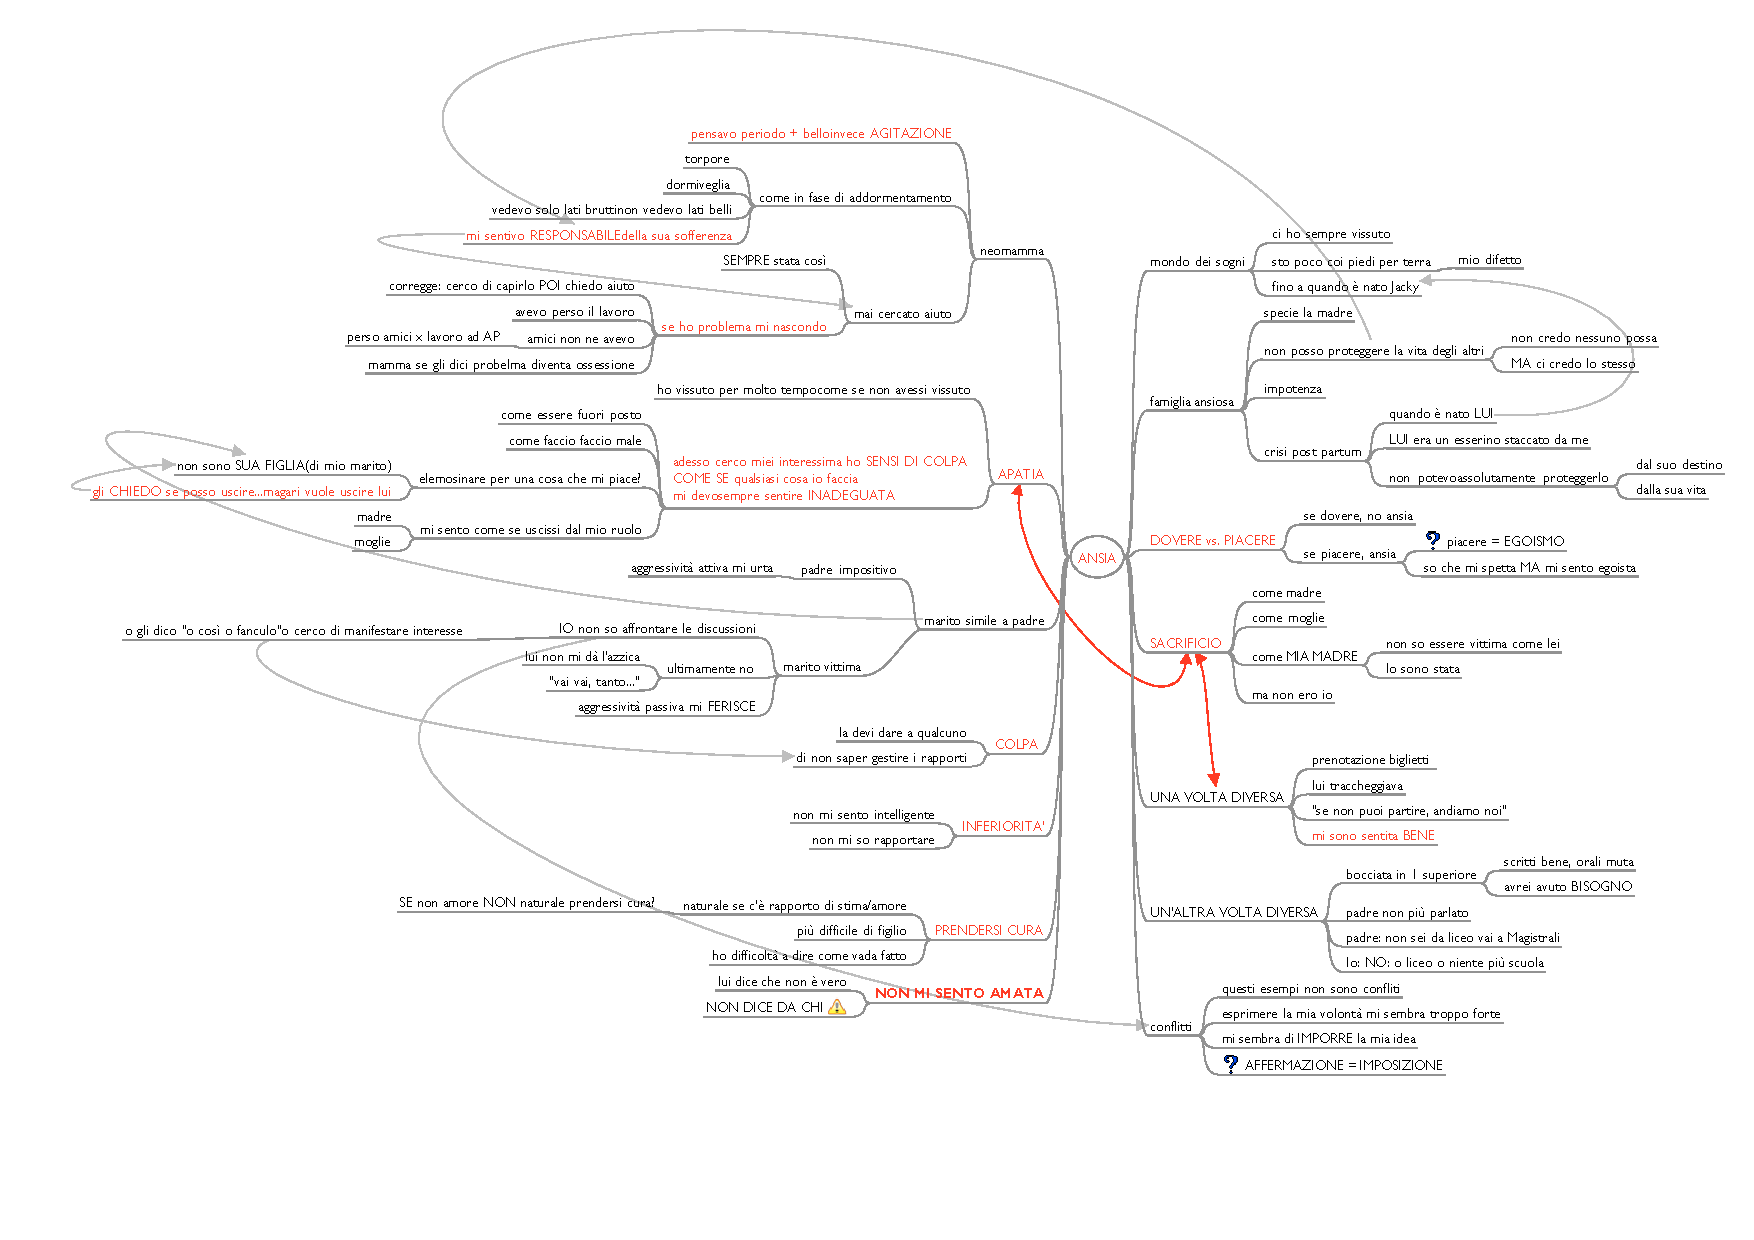
\includegraphics[angle=90,scale=1.5]{seduta1-2.pdf}
\end{fullwidth}
\end{figure}

\newpage
\section{Il terzo incontro}
\label{s:incontro3}
\subsection*{Sommario}

All'arrivo S. dice nuovamente di non avere temi nuovi di cui vuole parlare. Concordiamo perciò di riprendere il filo del discorso da dove lo avevamo lasciato. Dopo una breve \index{tematizzazione}tematizzazione dei contenuti dell'incontro precedente, riprendiamo la ricerca di un livello intermedio fra ''subire'' e ''imporsi'', che permetta a S. di esprimere in modo assertivo le proprie esigenze, rompendo il gioco copionico con il \index{marito!gioco copionico con}marito che abbiamo identificato nel precedente incontro.

Una volta accertata l'esistenza di questo livello intermedio, e la volontà di S. di percorrerlo, porto il discorso sulla scelta di un contesto in cui questo possa avvenire. Chiedo quindi a S. di esprimere un bisogno che vorrebbe affermare in maniera assertiva\index{assertivo!comportamento}. S. decide di voler ottenere del tempo per sé. Definiamo quindi questo come \index{obiettivo!definizione}obiettivo, ci accertiamo che sia ben formato, indichiamo un intervallo di tempo in cui raggiungerlo e concludiamo la seduta con l'assegnazione di un compito: S., entro il prossimo incontro, chiederà al \index{marito}marito del tempo per sé, e lo farà in maniera assertiva, per spezzare il gioco copionico.


\subsection*{Frasi salienti}

Investigando l'esistenza per S. di una alternativa rispetto alla \index{polarità} polarità \emph{elemosinare/imporsi}, S. gradualmente ristruttura la propria visione polare ammettendo l'esistenza di un livello intermedio, nel quale lei è in grado di esprimere i propri desideri senza arrivare a un conflitto e allo stesso tempo senza rinunciare a priori alle proprie richieste. 

Con l'occasione, S. individua anche una propria esigenza che da molto tempo rimane insoddisfatta, e che potrebbe costituire il problema da cui S. generalizza la propria convinzione di essere ''incapace'' e ''inadeguata'' nei rapporti.

\begin{verse}
C: \ldots{}prima hai detto che ti sembra di dover elemosinare; ora parli di importi. Sai immaginare un livello intermedio, dove non elemosini ma dove non ti imponi?\\
S: beh sì, dovrei dire quello che voglio fare e parlarne\\
C: per esempio di che cosa vorresti parlare senza problemi?\\
S: ah beh, del fatto che ho bisogno di uscire qualche volta\\
C: in che senso uscire?\\
S: nel senso che una sera ogni tanto vorrei vedermi con un'amica, o andare a fare spese, o al cinema, anche solo a fare una passeggiata, avere del tempo per me che  fra il lavoro, porta e riprendi i bambini, i mestieri, da mangiare e il resto, non ho mai un minuto per me da sola\\
C: e ti piacerebbe \emph{prenderti un tuo spazio}, solo per te?\\
S: ah, da morire!\\
C: c'è qualcosa che ti impedisce di farlo?\\
S: [pausa]
\end{verse}

\noindent A questo punto, \index{rispecchiamento}\index{ricalco-guida}\index{empatia!corporea} S. smette di parlare per qualche minuto. Dapprima, da appoggiata che era allo schienale, assume una posizione più rigida, in cima alla sedia, con i gomiti piantati; comincia a tormentarsi le mani e a respirare in modo un po' più accelerato. Inizialmente rispecchio la sua posizione in cima alla sedia, ma poi volutamente rispondo ai suoi movimenti con movimenti appena più lenti, e misurati; dapprima in modo impercettibile, poi sempre più evidente. Infine con un gran respiro mi appoggiato di nuovo allo schienale. Dopo qualche secondo, S. fa anche lei un gran respiro, si appoggia e riprende a parlare.\marginnote{Nel corso di questa parte del dialogo, in tutte le parafrasi cambio la parola \emph{chiedere} con la parola \emph{dire}; un piccolo \emph{ricalco-guida verbale} \index{ricalco-guida} per favorire la presa di coscienza della differenza fra un permesso concesso e un accordo fra pari; nel giro di poco, S. comincia anche lei a esprimersi nei termini di \emph{dire} anziché di \emph{chiedere}.}

\begin{verse}
S: quello che mi impedisce di farlo è il timore che poi finiamo come al solito\\
C: cosa intendi con ''come al solito''?\\
S: che lui mi dice ''sì, sì, vai, tanto\dots'' e a quel punto io sbotto, lo mando affanculo e non esco\\
C: tu con quali parole glielo chiedi? Puoi farmi un esempio?\\
S: beh, intanto gli chiedo se deve uscire\\
C: sì\dots\\
S: poi lui mi chiede perché, e a me già mi viene l'ansia\index{ansia}\dots poi gli dico che se non deve uscire magari potrei uscire io\dots\\
C: questo è il ''gioco'' di cui abbiamo parlato la volta scorsa, ricordi?\\
S: sì, assolutamente, ma vedi che ci ricasco\ldots\\
C: non è detto che debba succedere, abbiamo visto che c'è un meccanismo preciso che puoi interrompere; dimmi, come ti senti quando fai questo genere di richieste a tuo \index{marito}marito?\\
S: molto ansiosa\\
C: e quando devi \emph{dirgli} qualcosa, che so, ''abbiamo finito il latte, vai a prenderne un litro'', gli chiedi sempre prima se ha altri programmi?\\
S: no, in quel caso no. Se ha altri programmi me lo dirà lui\\
C: invece quando si tratta di chiedere qualcosa che riguarda te\dots\\
S: è vero, in quel caso è come se io gli chiedessi il permesso\\
C: credi di dovergli chiedere il permesso per uscire?\\
S: beh no, non sono mica sua \index{figlia}figlia\\
C: infatti, sei sua moglie. Ma allora, non ti sembra che gli \emph{chiedi} le cose come se volessi il suo permesso?\\
S: beh sì, è proprio così. E mi dà fastidio dovergli chiedere il permesso\\
C: come potresti fare a \emph{dirgli} che vuoi uscire senza che suoni come chiedergli il permesso?\\
S: beh, potrei dirglielo con un certo anticipo, così magari non ha già fatto altri programmi\\
C: e in che modo lo diresti, con quali parole?\\
\end{verse}

\noindent Qui S. fa una lunga pausa. \index{rispecchiamento}\index{ricalco-guida}\index{empatia!corporea} Assume di nuovo la posizione ''in punta di sedia'', ma io rimango appoggiato allo schienale, come se fossi del tutto rilassato e privo di fretta, senza fare movimenti o cenni che possano sollecitare una qualche risposta alla domanda in sospeso. Restiamo in silenzio per alcuni minuti, nel corso dei quali S. torna a una posizione più radicata sulla sedia e a movimenti più lenti. Poi riprende a parlare:

\begin{verse}
S: direi ''guarda, la sera tale vorrei prendermela per me, voglio uscire con le mie amiche''. Magari potrei dire che mi prendi una sera la settimana, come fa lui con gli amici?\\
C: lo stai chiedendo a me?\\
S: [ride] o madonna lo vedi, se non me lo facevi notare ci ricasco ancora; no  no che non lo sto chiedendo a te se posso, quello che voglio dire è che vorrei chiedere a mio \index{marito}marito del tempo per me, ma ''chiedere'' nel senso di dirglielo, non nel senso di avere il suo permesso, io \ldots{} io non voglio più avere bisogno del suo permesso\\
C: quindi ti senti di potere chiedere una cosa del genere\ldots\\
S: beh direi di sì, sì certo che posso; gli direi ''senti, tu il venerdì esci con gli amici, io voglio prendermi la sera del giovedì per me''. Ecco, gli direi così\\
C: bene; come ti farebbe sentire esprimerti in questo modo?\\
S: se ci penso, non mi sento in ansia\index{ansia}. Mi fà un po' strano perché è una cosa che non ho mai fatto, ma non mi dà l'angoscia.\\
\end{verse}

\noindent Ora provo a vedere se S. desidera, e si sente in grado di, passare dal discorso ipotetico alla definizione di un \index{obiettivo!definizione del}obiettivo reale, e alla buona formazione di questo obiettivo. In quest'ultima parte \index{ricalco-guida}, uso sempre il verbo ''dire'' (che non presuppone una concessione) al posto del verbo ''chiedere'', che invece S. usa ancora.

\begin{verse}
C: cosa ne pensi, ti piacerebbe darti proprio questa cosa come primo obiettivo?\\
S: ah, molto. Io non esco mai, ma mai mai, e mio \index{marito}marito non capisce che ho bisogno anche io di tempo per me\\
C: quindi per te è molto importante tanto l'avere del tempo per te quanto che tuo \index{marito}marito capisca?\\
S: beh\ldots io vorrei che lui capisse che non lo faccio per egoismo\ldots\\
C: e se per caso lui non capisce? Che cosa è veramente importante per te?\\
S: [lunga pausa] se lui non capisce\ldots lo capirà più avanti, io così non posso continuare\\
C: bene, allora vuoi \emph{dirgli} che vuoi del tempo per te?\\ 
S: sì\\
C: se ti prendi questo tempo per te, qualcuno ne avrà un danno?\\
S: no, i ragazzi possono stare a casa una sera con lui, è già successo altre volte\\
C: bene, quanto tempo per te vorresti, esattamente?\\
S: vorrei ritagliarmi una sera alla settimana tutta per me. Anche se non so ancora cosa ci farò tutte le volte\\
C: questo potrai deciderlo di volta in volta. In che modo pensi di dirglielo?\\
S: come abbiamo detto adesso. Con una settimana di preavviso, diciamo\\
C: e quando penseresti di farlo?\\
S: eeeeh\dots magari fra un paio di settimane?\\
C: perché non provi invece a \emph{dirlo} questa settimana per la prossima? Pensi di poterlo fare?\\
S: oddio, non ho mai detto una cosa del genere\dots\\
C: puoi semplicemente \emph{dirlo} come lo hai detto a me\\
S: ma non sono sicura di riuscirci\ldots\\
C: quello è un altro problema; per questa volta \index{obiettivo!definizione del}l'obiettivo è \emph{dire} ciò che vuoi; te la senti?\\
S: sì\\
C: che sera scegli?\\
S: mi piacerebbe il giovedì\\
C: bene, vada per il giovedì; puoi \emph{dirglielo} prima che finisca questa settimana?\\
S: beh\ldots sì\\
C: come ti sentirai dopo averglielo detto?\\
S: se ci riesco sarà bellissimo, mi sentirò molto sollevata\\
C: e se ti dice di no cosa rispondi?\\
S: [ride] lo mando affanculo? [pausa] No no\ldots ci devo pensare, gli dico che ci devo pensare\\
C: pensi di avere necessità di valutare in anticipo come reagire a una sua eventuale risposta negativa?\\
S: [pausa] beh no, non proprio. Posso sempre cavarmela dicendo che dovremo riparlarne meglio; lui non ne farà una questione\\
C:  bene, allora cosa ne dici provare a dirglielo questa settimana, come dicevi? Se poi invece non te la senti, possiamo riparlarne la prossima volta e valutare cosa potrebbe succedere nel caso che lui si opponga. Che ne dici?\\
S: ah, mi piace così\\
C: bene, allora siamo d'accordo? Ti prendi questa responsabilità?\\
S: sì.\\
\end{verse}

\noindent Chiudo l'incontro con una breve \index{tematizzazione}tematizzazione riassuntiva di quanto ci siamo detti, e quando arrivo alla consegna chiedo che S. la ripeta con parole sue, cosa che sembra darle una certa soddisfazione.

 


\newpage
\section{Il quarto incontro}
\label{s:incontro4}
\subsection*{Sommario}
 
L'incontro si apre con la notizia del raggiungimento \index{obiettivo!raggiungimento}dell'obiettivo concordato durante l'incontro precedente: S. ha detto al \index{marito}marito che d'ora in poi prenderà per sé la serata del giovedì. S. si dice molto contenta del risultato e quasi incredula della facilità con cui lo ha raggiunto. Ha evidentemente un forte interesse a condividere questa sua esperienza, e faccio in modo che si prenda tutto il tempo e il livello di dettaglio che desidera.
Il racconto di ciò che è avvenuto, e di come S. si sia sentita prima e dopo il colloquio e di come si senta adesso occupa tutto l'incontro.

\subsection*{Frasi salienti}

\begin{verse}
C: ricordo che ci eravamo dati una consegna per oggi, no?\\
S: sì sì\ldots\\
C: vuoi dirmi come è andata?\\
S: guarda, all'inizio non volevo nemmeno dirglielo perché non sapevo come iniziare il discorso, volevo tornare qui e dirti che non ero pronta\ldots{}Poi una sera siamo entrati in argomento, e mi sono detta ''beh, adesso o mai più'' e gliel'ho detto, gli ho detto ''senti, ho deciso che il giovedì è la mia sera libera, come il venerdì per te''\\
C: e lui come ha reagito?\\
S: mah, ha avuto un attimo come se fosse stupito, poi ha detto ''ah ok, va bene'' ed è stato tutto, davvero, avremo parlato forse due minuti in tutto\ldots{}\\
\ldots\\
C: prima di parlargli come ti sentivi?\\
S: molto nervosa\ldots{}i primi due giorni pensavo di non farcela, poi di non trovare l'occasione, poi che sarebbe finita come al solito, ti dico, volevo tornare e dirti che non ero pronta\ldots{}poi però pensavo anche che in fondo non chiedevo niente di sbagliato, e soprattutto che ora che avevamo individuato il gioco ero libera di non ricaderci, quindi tutto sommato volevo tentare\ldots{}così anche se ero molto nervosa, facevo le prove da sola di quello che dovevo dire\ldots{}\\
C: possiamo dire che hai ''provato le battute''? \\
S: sì, le ho provate prima un tot di volte, solo che all'inizio mi mancava un po' il fiato, poi invece mi sono detta che non dovevo mica stare lì a fare tanti discorsi e perché e percome, e quando c'è stata l'occasione non sono stata lì a pensarci troppo, sono andata dritta al sodo e le parole mi sono venute con naturalezza\\
\ldots{}\\
C: come ti sei sentita dopo il colloquio?\\
S: beh sono andata in cucina perché non mi vedesse, mi veniva quasi da ridere dalla contentezza\ldots{}non mi sembrava vero che fosse stato così facile
\end{verse}

\noindent Il colloquio prosegue a lungo su questa linea, perché S. si esprime con molta energia; accolgo il suo racconto con interesse, perché senta accettazione e approvazione per lo sforzo effettuato e l'ottimo risultato.

Dopo che il racconto si è esaurito, chiedo a S. se abbia già usufruito di questa conquistata ''finestra di autonomia''; la richiesta del giovedì libero al \index{marito}marito risale al mercoledì, quindi S. ha già avuto un'occasione per sperimentare un proprio momento di autonomia. Mi chiedo, e le chiedo, se l'ha sfruttata.

\begin{verse}
C: hai già avuto occasione di prenderti il tuo giovedì sera?\\
S: sì, la sera dopo, che era giovedì\\
C: me ne vuoi parlare?\\
S: ma guarda, al pomeriggio mi sono sentita con un'amica, una che non vedevo da un sacco di tempo, a un certo punto mi fa ''dai, ma vediamoci una sera che facciamo una girata in città'' e a quel punto le ho detto ''ma guarda, io posso il giovedì, tu come sei messa?'' e insomma, lei era libera e quindi dopocena ci siamo viste\\
C: come ti sei sentita quando lo hai detto a tuo \index{marito}marito?\\
S: beh all'inizio titubavo un po', non sapevo come metterla, no? Poi ho pensato come ci eravamo detti, che la parte difficile era stabilire la regola, che anche io mi posso prendere una sera la settimana, che poi magari non so neanche cosa fare tutte le settimane però poi al massimo dico ''ecco, questa settimana scelgo di stare a casa'', non è una cosa che subisco, la mia sera ce l'ho, se mi va me la prendo e se no resto a casa\ldots\\
\ldots\\
S: comunque insomma, lui è arrivato, e come è andata oggi e l'ufficio\ldots{}e poi dopo i convenevoli gli ho fatto:''senti, oggi è giovedì, io uscirei con la Gianna'', gliel'ho detto così, come una cosa normale\ldots\\
C: e infatti era  una cosa normale, lo avevate concordato il giorno prima\ldots\\
S: proprio così. E infatti lui non ha battuto ciglio, ha detto ''ah sì sì, a che ora esci?'' e finita lì
C: come ti sei sentita dopo averglielo detto?\\
S: mah, benone, ti dico, è stata una cosa proprio normale, normalissima\ldots\\
C: e come ti ha fatto sentire, questa ''normalità''?\\
S: [pausa] beh guarda, in effetti ho pensato che se era così facile potevo pure pensarci prima, poi mi sono sentita\ldots{}contenta, ecco; contenta, ma proprio soddisfatta\\
C: mi parli un po' di questa contentezza?\\
S: beh, ero contenta perché intanto facevo una cosa a cui tenevo, no, uscire, avere del tempo per me\ldots{}ma poi proprio perché io non credevo che ci sarei riuscita, e men che meno senza litigate\ldots\\
C: possiamo dire che eri felice del tuo successo?\\
S: ah sì, assolutamente\\
C: e secondo te da cosa è dipeso questo successo?\\
S: mah, non era la prima volta che gli chiedevo una cosa del genere come sai\ldots{}però questa volta è stata diversa, gliel'ho detto
in modo diverso; voglio dire, che di solito iniziavo con un ''sono stanca'' oppure ''faccio sempre casa--ufficio ufficio--casa, ho bisogno di un po' d'aria'', o magari chiedendogli prima se lui aveva un impegno\ldots{}e a quel punto lui faceva sempre l'accomodante, mi diceva ''sì sì, esci pure, tanto\ldots'' e quello proprio mi mandava in bestia, guarda. A quel punto dicevo che se le cose stavano così non mi andava più di uscire, ma glielo urlavo, proprio, e lui lì con quel fare\ldots{}perché lui riusciva a far passare me per quella mezza isterica, no?\\
C: ho notato che riguardo a questa volta dici ''gliel'ho detto'', hai usato il verbo \emph{dire}; di solito usavi il verbo ''chiedere''\\
S: e infatti è proprio quello il punto! [sorride] Proprio lì sta la differenza, prima era sempre un chiedere, quasi a mendicare, no, e a me mi dava fastidio perché cosa devo chiederti, che in casa non sposti un piatto\ldots{}[pausa] Insomma, stavolta non gli ho chiesto il permesso, non ho nemmeno cercato di spiegargli che era giusto, perché insomma, \emph{è} giusto, lui si prende il suo tempo e io devo potermi prendere il mio, non è mica una ripicca!\\
C: se ti dicessi che hai avuto un comportamento assertivo\index{assertivo!comportamento} cosa ne penseresti?\\
S: penserei che è stato proprio così\\
C: hai detto che dicevi ''se le cose stavano così''; ma ''così'' come?\\
S: [lunga pausa] sì, è il gioco di cui abbiamo parlato l'altra volta, io partivo facendo la vittima e lui era il persecutore\ldots\\
C: e ti ricordi quale abbiamo concluso che fosse il tuo ''ritorno''?\\
S: che confermavo la mia convinzione di non essere OK, cioè preferivo una conferma negativa piuttosto che rischiare di fallire cercandone una positiva\\
\end{verse}

\noindent Arrivati allo scadere del tempo convenuto, sollecito la collaborazione di S. per una \index{tematizzazione}tematizzazione riassuntiva.
S. riconosce di essersi comportata in modo assertivo\index{assertivo!comportamento} e di avere potuto, grazie a questo atteggiamento, evitare di cadere nel gioco \index{gioco Berniano}Berniano che avevamo analizzato (vedi pag. \pageref{s:incontro2} e segg.). Il comportamento assertivo le ha permesso di ottenere un risultato per lei molto importante, e riconoscendo allo stesso tempo il meccanismo comunicativo in cui lei e il \index{marito}marito erano invischiati a propria insaputa. S. si dice anche felice del fatto che le cose si siano svolte in modo più semplice di ciò che si aspettava e che questo le è da stimolo per fare attenzioni in altre situazioni per riconoscere meccanismi simili. Concludiamo l'incontro senza l'assegnazione di homework.


\newpage
\section{Il quinto incontro}
\label{s:incontro5}
\subsection*{Sommario}
All'arrivo, richiesta se ci siano elementi nuovi, S. espone alcune difficoltà contingenti nei rapporti con il \index{figlio!secondo}figlio più piccolo: lo svolgimento dei compiti, e in particolare il rapporto con l'insegnante; di nuovo, nell'esporre queste difficoltà, S. indica la propria reazione come ''ansia''\index{costrutti!ansia} e \index{senso di inadeguatezza}''senso di inadeguatezza''. Il colloquio permette di avanzare l'ipotesi, che dovà venire esplorata, che alcuni problemi che S. attribuisce al figlio, come ad esempio i rapporti con l'insegnante, possano essere in realtà proiezioni di \index{svalutazioni}svalutazioni che S. fà riguardo a se stessa.
 
\newthought{Nel corso del colloquio} cerco di esplorare i vari aspetti del rapporto di S. con il \index{figlio!secondo!rapporti con}figlio e con la di lui insegnante, individuando alcune incongruenze fra quanto S. sostiene avvenire ''sempre'' e quanto, per sua ammissione, accade. Posta di fronte a queste apparenti incongruenze, S. nota delle differenze nelle proprie valutazioni, quando queste vengono fatte in modo istintivo e quando vengono prodotte in modo più ragionato. Infatti, le sue valutazioni riguardo a: 
\begin{itemize}
\item il rapporto con l'insegnante del \index{figlio!secondo!rapporti con}figlio minore
\item il suo timore di essere manchevole nei confronti del figlio minore
\end{itemize}
sono molto diverse nei due casi; la valutazione istintiva sembra suggerire una notevole problematicità, mentre la spiegazione della situazione non risulta altrettanto problematica. Verso la conclusione della seduta, inizio a ipotizzare che una parte dell'ansia\index{ansia} denunciata da S. possa forse dipendere dalle prime richieste di autonomia del figlio.

\subsection*{Frasi salienti}

\begin{verse}
S: vorrei tornare sulla mia inadeguatezza, sull'ansia\index{ansia}, perché me le ritrovo in situazioni diverse, nel senso, mi torna sempre come punto centrale dei miei comportamenti\ldots\\ cioè me lo sento molto forte in questi giorni\\
C: è successo qualcosa di particolare di cui vuoi parlare?\\
S: beh, ho il problema della scuola di mio \index{figlio!secondo}figlio piccolo, a parte il calcio, tutte le difficoltà\ldots{}purtroppo ha incontrato una professoressa di italiano \emph{terribile}, gli dà un fracasso di compiti, ma di compiti \emph{inutili}, nel senso gli dà una pagina del libro, dove ci sono gli esercizi da riempire, no? ecco, lì basterebbe scrivere le risposte, le crocette, e invece no, lei gli fa anche ricopiare tutta la pagina, ma gli dà pagine intere\ldots{}l'altro giorno siamo stati dalle due e mezza alle sette e mezza a fare i compiti di Italiano, e poi c'era ancora Storia\ldots\\
C: cinque ore per i soli compiti di italiano?\\
S: sì, ed è la seconda volta che ci capita 'sta cosa\ldots{}e io vado subito in ansia\index{ansia}\\
C: in ansia\ldots\\
S: sì, ma guarda, un'ansia da panico, quasi\\
C: e quale motivo ti dai per quest'ansia, a cosa credi sia dovuta?\\
S: eh, è dovuta al fatto che è colpa mia se lui è capitato in quella sezione, colpa mia che non sono stata attenta magari a iscrivelro in una scuola buona\ldots{}cioè, mi sento sempre inadeguata, mi sento sempre come di non essere una buona madre, che non si è informata sui professori che c'erano, che non è stata attenta, ha lasciato un po' le cose al caso\ldots{}cioè adesso non so come aiutarlo, cioè più che stargli vicina e aiutarlo, sostenerlo\ldots{}però mi sento quest'ansia dentro, forse magari perché forse vorrei risolvere la cosa subito, ma capisco che poi in realtà non si può risolvere subito\ldots\\
C: quindi vediamo se ho seguito tutto: lui ha tanti compiti; non riuscite a farli tutti quanti\ldots\\
S: lui mi fa in crisi, naturalmente, e vado in crisi pure io\\
C: ''va in crisi'' cosa significa?\\
S: che si mette a piangere, ''io non ce la faccio più'', e '' sono stanco''\ldots{}scene un po' \emph{isterichine}\ldots\\ e io purtroppo non so come fargli capire\ldots{}che non è nemmeno giusto che un bambino di quell'età passi dodici ore sui libri\\
\end{verse}

\noindent S. racconta di avere contattato altre mamme, anch'esse con problemi analoghi,  e di avere richiesto con loro un colloquio con il Preside. Le faccio notare che ciò significa che il problema non è un problema suo personale, e lo riconosce, ma replica:

\begin{verse}
S: però io non capisco perché devo avere sempre questa morsa allo stomaco\ldots{}come una cinghia, ecco\ldots{}forse è proprio vero che ho troppa fretta di risolvere le cose, gli dò troppo peso, e invece dovrei \emph{aspettaaare, valutaaare} e poi trovare magari le risoluzioni, senza che mi venga 'sto groppo\ldots{}no?\\
C: che cosa potrebbe essere una soluzione?\\
S: di soluzioni ce ne sono tante, parlare con la professoressa, col Preside, vedere come vanno le cose, e al massimo spostarlo di classe\\
C: direi che hai non una sola, ma un ventaglio di soluzioni possibili, tu come la vedi?\label{ventaglio}\\
S: sì, ce ne sono tante in teoria, ma poi\ldots{} se ci sono tutte queste soluzioni perché io devo avere questo groppo, questa cinghia che mi strizza lo stomaco?\\ 
\end{verse}

\noindent Il colloquio prosegue cercando altre occasioni in cui questa sensazione si manifesta:i problemi di scuola del \index{figlio!secondo}figlio, oppure sul lavoro. Dal racconto di S. sembra che questa ansia\index{ansia} sia la sua reazione automatica a \emph{qualsiasi} situazione problematica, e infatti lei sostiene proprio questo:
\begin{verse}
S: sempre, quando io ho un problema ho questo \emph{peso}\ldots{}e mi disturba anche molto perché le soluzioni le vedo, non capisco perché mi pesa così
\end{verse}

\noindent A questo punto chiedo a S. di ricordare situazioni, anch'esse problematiche, in cui però questo peso non si sia manifestato. S. ci pensa un po'.

\begin{verse}
S: il peso non c'è quando il problema lo posso risolvere con una \emph{azione determinata}, in un tempo determinato, no? Tipo: ho il problema, faccio la tal cosa, risolvo, tac--tac--tac\\
C: puoi farmi qualche esempio?\\
S: ma tipo: metti che mio \index{figlio!secondo}figlio si ammala, tipo ha una brutta tosse:  sento il dottore, glielo porto, finisce lì, nessun peso, nessuna ansia\index{ansia}; o quando ho fatto l'incidente con la macchina, ho avuto sì paura, ma ansia no, ho pensato: ''porto la macchina dal meccanico, non mi sono fatta male, basta''. Forse è perché è tutto molto rapido, no, il passaggio dal problema alla soluzione\ldots\\
C: forse, però prendi l'esempio della brutta tosse, magari il dottore ti dice ''gli dia questo, lo tenga a casa magari una settimana''; o quando hai avuto l'incidente: hai portato la macchina a riparare ma sei rimasta a piedi per quindici giorni, mi dicevi. E l'insegnante di tuo \index{figlio!secondo}figlio la incontrate proprio fra una settimana. Quindi l'intervallo di tempo in cui il problema sussiste è lo stesso. Che cosa c'è di diverso in questo incontro con l'insegnante che non c'è nell'avere il bimbo malato, o la macchina dal meccanico?\\
S: [pausa] c'è\ldots{}che negli altri casi io è come se delegassi la \index{responsabilità}responsabilità\ldots{}il dottore mi dice cosa fare, il meccanico ripara\ldots{}con l'insegnante invece  io devo mettermi in relazione, spiegare, criticare, non come una critica, ma per farle capire che insomma non è giusto anche per i bambini\ldots{}ecco, io \emph{non mi reputo capace} di spiegare a questa persona che non conosco, non so poi come la prende, io in questo caso non ho nessuna via d'uscita possibile\ldots
\end{verse}

\noindent La matrice di svalutazione\index{svalutazione!matrice di} (v. pag. \pageref{tab:svalutazione}) dell'AT\index{Analisi Transazionale} aiuta ad illustrare la situazione attuale:
\begin{enumerate}
\item S. riconosce l'esistenza di segnali che indicano una situazione di problema: quindi non svaluta l'esistenza degli stimoli né l'esistenza del problema (diagonali 1 e 2)
\item si sente in grado di riconoscere ulteriori segnali di evoluzione della situazione, quindi non sta svalutando la propria possibilità di reagire agli stimoli (diagonale 3)
\item sa di poter fare fronte a determinate situazioni  problematiche (diagonale 4), quindi non sta svalutando la propria possibilità di agire sui problemi
\item per contro, S. svaluta la propria \emph{possibilità} di individuare soluzioni possibili e di agire su questo specifico problema (diagonale 5)
\item lo strumento della matrice di svalutazione ci dice anche che S. svaluta la propria capacità di mettere in atto eventuali soluzioni suggerite (diagonale 6)
\end{enumerate}

\noindent Secondo la matrice di svalutazione, non ha senso intervenire suggerendo una modalità di comportamento (diagonale 6), perché S. comunque svaluta la propria \emph{possibilità} di individuare soluzioni e la propria capacità di metterle in atto (diagonale 5). Secondo l'AT, il livello corretto a cui intervenire è proprio questo, aiutare S. a:

\begin{enumerate}
\item scoprirsi in grado di immaginare soluzioni possibili
\item scoprirsi in grado di metterle in atto
\end{enumerate}

\noindent Mostro a S. la \index{svalutazione!matrice di}matrice di svalutazione e dove si collocano le sue affermazioni di questo incontro e dei precedenti relative al nuovo problema emerso. Le mostro anche che determinate ''conseguenze'' previste dalla matrice (se si svaluta $x_ij$ si svalutano anche tutte le caselle sulla stessa diagonale e quelle sottostanti) corrispondono a ciò che lei racconta di sé. Giunti nuovamente al termine del tempo stabilito, procedo a una \index{tematizzazione}tematizzazione riassuntiva e all'indicazione di come potremo procedere nei prossimi incontri.

\begin{verse}
C: allora, questa volta mi hai parlato di un problema con tuo \index{figlio!secondo}figlio, nello specifico con la professoressa di Italiano; il problema consiste nel fatto che l'insegnante secondo te assegna troppi compiti, e tu provi ansia\index{ansia} e senso di inadeguatezza all'idea di relazionarti con lei e spiegarle\ldots\\
S: sì, esatto\\
C: e abbiamo anche visto come, dalle tue parole, uno strumento dell'AT ci dice che tu, pur riconoscendo che esistono delle soluzioni, stai svalutando la tua capacità di vederle riferite a te, e stai svalutando anche la tua capacità di agire per metterle in atto\\
S: proprio così, io non mi vedo in grado di superare questo problema\\
C: ecco, nel prossimo incontro, se vuoi, ripartiremo proprio da qui: immagineremo assieme varie modalità di comportamento e vedremo se, in fin dei conti, non possano rivelarsi positive per risolvere questo problema. Magari potresti cominciare a pensare a qualche possibilità, sia che ti sembri funzionare sia che no, e la prossima volta ne possiamo parlare. Sei d'accordo?\\
S: ok, va bene\\
\end{verse}

\subsection*{Elementi di contro-transfert}\index{controtransfert}
\begin{itemize}
\item \textsl{Cosa ho sentito}\\
Durante l'incontro precedente, ho avvertito in due occasioni l'istinto di colludere con S. 
\begin{enumerate}
\item quando S. ha menzionato la professoressa ''terribile'' ho avuto l'istinto di dire ''hai proprio ragione''
\item alla menzione del ''groppo'' e della ''cinghia che strizza'' lo stomaco, ho avvertito la stessa sensazione e ho ricordato che mi è stata e mi è familiare
\end{enumerate}

\item \textsl{Perché l'ho sentito}\\
Le mie sensazioni sono state dovute al riconoscere parte della mia personale esperienza nel racconto di S.
\begin{enumerate}
\item durante il percorso di studi mi è capitato spesso di entrare in conflitto con insegnanti che valutavo impreparati, scorretti o non abili nel gestire l'aula; per questo mi sono riconosciuto nel racconto di S. 
\item mi è capitato e tuttora talvolta mi capita di avere quel tipo di reazione fisica quando mi trovo di fronte a situazioni che mi sembrano al di là della mia portata; specialmente nel passato, in quei momenti, ho seguito istinti di evitamento o di conclusione affrettata, spesso a mio svantaggio.
\end{enumerate}

\item \textsl{La mia strategia di coping}\index{coping}\\
Sono riuscito a fare fronte a questi due istinti collusivi grazie al fatto che si sono manifestati in modo molto evidente come tali, e quindi ho potuto riconoscerli e mettere in atto in ciascun caso una modalità di \emph{coping}:
\begin{enumerate}
\item la reazione del counselor che dice ''hai proprio ragione'' è così canonicamente \index{collusione}collusiva che non ho potuto non accorgermene in tempo. Questo mi ha permesso di non seguire l'istinto e invece di portare la mia attenzione sulla situazione che S. stava descrivendo, e soprattutto di ricordare a me stesso che quella descritta non era la situazione oggettiva, ma la situazione come lei la stava vivendo; ho pertanto annotato di investigare la situazione ''compiti eccessivi'' per consentire, anche a S., di valutare il punto di vista dell'insegnante e il proprio ruolo nel problema
\item l'associazione fra sensazione corporea e istinto di \index{evitamento}evitamento fa parte del mio vissuto,  non di quello della cliente. Pertanto, ho annotato di investigare a quale tipo di pensiero lei associ questa sensazione. Ho anche ottenuto di rendere meno intensa la mia sensazione invitando la cliente a fornire maggiori dettagli sul contesto in cui questa si verifichi; l'alienità di questo contesto mi ha permesso di riguadagnare una certa distanza emotiva dal racconto.
\end{enumerate}
\end{itemize}


\newpage
\section{Il sesto incontro}
\label{s:incontro6}
\subsection*{Sommario}
Poiché S. non ha portato nuove problematiche, in questo incontro abbiamo continuato ad investigare il problema dei compiti assegnati dalla professoressa di Italiano al \index{figlio!secondo}figlio più piccolo, compiti che S. ritiene ''eccessivi''.
All'inizio, per iniziare a lavorare sulle \index{svalutazioni}svalutazioni, ho chiesto a S. di immaginare cosa potrebbe dire alla professoressa ossia, ho chiesto a S. di ipotizzare possibili soluzioni, di cui conosce e ammette l'esistenza ma che non ritiene di potere e di sapere applicare.

Durante il colloquio S. ha poi ripetutamente cambiato il nome della propria sensazione da ''ansia''\index{costrutti!ansia} a \index{costrutti!paura}''paura'', e abbiamo quindi cercato di investigare a cosa questa paura sia riferita. Individuato \index{elastico} l'\emph{elastico} di una precedente esperienza di S., proseguiamo investigando se c'è qualcosa, nel comportamento attuale di S., che la metta in condizioni di sperimentare l'\emph{elastico} dell'esperienza problematica vissuta in passato. Una volta trovato un comportamento che sembra essere scatenante, valutiamo i motivi che danno origine questo comportamento; l'incontro si chiude annotando di dedicare l'incontro successivo, assente l'insorgenza di problemi contingenti, a una riflessione sulla opportunità di proseguire o di modificare questo comportamento.

\subsection*{Frasi salienti}

All'inizio del colloquio, chiedo a S. se ricorda che nel precedente incontro ha ipotizzato diversi modi di intavolare la discussione con la professoressa\sidenote{si veda pag. \pageref{ventaglio}} e la invito a parlarmene:
\begin{verse}
C: bene, allora visto che non ci sono novità oggi lavoriamo un po' sulle opzioni che hai a disposizione; ricordi che la volta scorsa hai elencato  diverse possibili soluzioni al problema?\\
S: sì, me lo ricordo, dal risolvere tutto parlando con la prof fino al cambiare classe\ldots\\
C: mi vuoi dire come potresti parlare con la professoressa, cosa potresti dirle durante l'incontro che avrete?\\
S: beh\ldots{}intanto le farei notare che stiamo parlando di bambini, sono usciti sei mesi fa dalle elementari\ldots{}lei dovrebbe non lo so, capire cosa sanno, dargli tempo di adattarsi\ldots{}e poi certo, io penso che ''il più'' debba essere fatto a scuola, ecco, poi a casa ripassi, certo, ma non così\ldots\\
C: ma secondo te, che motivo può avere l'insegnante per assegnare compiti in questa quantità che trovi eccessiva?\\
S: mah, non lo so\ldots\\
C: cosa ne pensi del fatto che la scrittura sia anche una capacità manuale, a cui allenarsi, tu cosa ne pensi?\\
S: beh sì, scrivono ancora come bambini delle elementari, ma io quando ho visto le tre pagine da ricopiare\ldots{}mi ha spaventato, ecco, ho avuto paura che questa persona non sia stabile, paura per lui\\
C: ma paura per che cosa esattamente?\\
S: [lunga pausa] mah\ldots{}credo\ldots{}non so, che non \emph{mi} [enfasi mia, NdA] regga tutti questi stress\ldots\\
C: però mi hai detto che la paura è tua, non sua\ldots\\
S: già, è vero\ldots{}sono io che ho paura\ldots{}ma perché?\\
\end{verse}

\noindent La sensazione di paura viene ripetuta più volte quando chiedo a S. di dettagliare ulteriormente la sua situazione riguardo ai compiti assegnati. Analizzo con S. come la paura non sia una reazione congrua rispetto alla situazione, e le chiedo se vede qualche analogia con qualche esperienza del suo passato.

\begin{verse}
S: [pausa] dunque\ldots{}alle elementari zero, avevo buoni insegnanti; alle medie\ldots{}quella di Italiano era proprio brava, si vedeva che aveva la passione, e ce la trasmetteva, quando ci leggeva eravamo come rapiti\ldots{}se devo proprio ricordare un'insegnante terribile, ecco, quella di danza, quella era proprio pazza secondo me, urlava, ti tirava le cose\ldots{}che poi a me quando mi urli vado in confusione, faccio tutto il contrario di quello che mi dicono, tipo lei mi urlava ''vai a destra!!!'' e io andavo in confusione e andavo a sinistra\ldots\\
\end{verse}

Con S. parliamo di come la situazione passata con l'insegnante di danza sembri costituire un \index{elastico}\emph{elastico} con la situazione attuale. In pratica, S. ha paura non dell'attuale insegnante di Italiano del \index{figlio!secondo}figlio, ma della sua vecchia insegnante di danza, e la paura è che quella si manifesti di nuovo in questa. S. riconosce che ci sono delle differenze, ma insiste che ci sono anche delle affinità. Questo mi dà l'occasione di riportare il figlio nel discorso, poiché è della sua insegnante e dei suoi compiti che stiamo parlando.

\begin{verse}
S: beh quella [l'insegnante di danza, NdA] era letteralmente una pazza, una disturbata, ci tirava addosso di tutto\ldots{}questa di Italiano non è a quei livelli, però ho saputo da una mamma che ha tirato un quaderno a un bambino che aveva sbagliato un compito\ldots\\
C: beh certo una cosa del genere, se fosse verificata, giustificherebbe i tuoi timori. Però, mi viene da dire: e tuo figlio, che cosa ne pensa di quest'insegnante?\\
S: ma guarda, questa è bella perché lui, vedi, la giustifica\ldots{}tipo l'altro giorno, con tutti quei compiti, io davo in escandescenze per quanti erano e lui mi fa ''ma mamma, ce li avrà dati per prepararci, che sabato abbiamo la verifica, no?''; ti dico, sono rimasta un attimo interdetta\\
C: e a parte i compiti, lui cosa ne pensa di questa insegnante?\\
S: a lui piace, perfino. Quando gli ho chiesto come ci si trova lui mi ha detto ''mamma, devi sentire come legge per noi, stiamo tutti lì zitti zitti''\\
C: mi ricordo che anche tu mi hai detto di aver avuto una insegnante che quando leggeva restavate come rapiti\ldots\\
S: sì, è vero, ora che me lo fai notare ha detto la stessa cosa che ho detto io, è incredibile\\
\end{verse}

\noindent Proseguiamo il colloquio con S. che confronta a lungo i propri rapporti con la vecchia insegnante di danza e, dall'altro lato, i rapporti del \index{figlio!secondo}figlio con l'attuale insegnante di Italiano. Alla fine S. riconosce spontaneamente, seguendo il filo del proprio ragionamento, che non è il figlio, ma lei stessa ad esprimere difficoltà verso l'insegnante di Italiano. Il dialogo prosegue con S. che riporta i problemi del figlio a un proprio trauma infantile, e ipotizza che sia quel trauma il vero \index{elastico}elastico che le causa queste relazioni non congruenti.

\begin{verse}
S: perché, per dire, non so come rapportarmi con lei senza magari eccedere in aggressività\\
C: ma temi di essere tu troppo aggressiva o che lo sia lei?\\
S: eh se lo fosse lei, metti che si mettesse a urlare, a dirmi ''suo figlio non capisce niente, lei non lo segue abbastanza'', sarei costretta a cambiarlo di classe, e questo per me sarebbe molto più un trauma, perché dovrei spostarlo da un ambiente dove conosce tutti a uno dove non conosce nessuno, e lui non ama queste cose, non è molto molto socievole, non si adatta molto facilmente agli ambienti nuovi\ldots\\
C: te lo ha detto lui questo?\\
S: mah, sì, ha detto, che se magari conoscesse già qualche altro bambino sarebbe , lui cerca sempre un aggancio di qualcuno che conosce, però ecco, all'inizio\ldots{}anche se poi non penso che avrebbe grossi problemi tranne all'inizio\ldots{}perché l'ha fatto, cioè questa cosa l'ho fatta: quando ha cominciato a giocare a calcio, non l'ho iscritto alla società vicino casa, perché si sarebbe ritrovato tutti  i bambini con cui andava all'asilo, da tanti anni, a scuola\ldots{}e siccome è un bambino che ha di queste difficoltà, ho detto no, proviamo a fargli cambiare e a fargli conoscere un ambiente nuovo. E quindi all'inizio ho parlato con l'allenatore, gli ho chiesto di cercare di \index{coinvolgimento}coinvolgerlo\ldots{}e alla fine si è inserito bene, però comunque è uno che ha i suoi tempi, le sue particolarità, non è quello sempre compagnone, però essendo piccolo, insomma, è normale\\
C: da quello che mi dici mi sembra un bambino con delle risorse, comunque\\
S: sì, perché anche lui magari ha più paura nel pensarlo che nel farlo [pausa] beh,\emph{ io in questo\ldots{}purtroppo\ldots} [enfasi mia]\\
C: tu hai traslocato spesso da bambina?\\
S: ehh\ldots{}io ho traslocato una volta e\ldots{}è stato un trauma per me\\
C: quanti anni avevi?\\
S: avevo undici anni, da S. Maria di Loreto sono passata a\ldots{}vicino a Santa Veneranda, e a quell'epoca era tutto campi, io pensavo di avere cambiato città, addirittura, perché mia mamma non mi mandava in città con la bici, a parte che non sarei riuscita ad arrivarci, mi sarei persa\ldots{}io ci sono stata molto male, ci ho sofferto molto. Però, sai che non me lo ricordavo?\\
C: però nel caso di tuo figlio, se anche per estremo dovesse cambiare classe o scuola, non sarebbe la stessa cosa che è stata per te, lui avrebbe sempre la squadra di calcio\\
S: eh, il problema è che è più insopportabile per me che per lui\\
C: però non sei tu che devi andare a scuola\ldots\\
S: eh, ma io ho sofferto tanto, tantissimo per la scuola, perché a me non piaceva andare a scuola, e da me si aspettavano sempre tanto, chissà perché poi, e io non ho mai dato tanto\\
C: non hai una laurea in Legge?\\
S: sì, però prima di arrivarci\ldots\\
C: hai ripetuto un anno?\\
S: ripetuto un anno, poi sono sempre stata rimandata, al Liceo\ldots{}comunque li ho fatti patire, soprattutto mia mamma che viveva questa cosa con molta molta angoscia [pausa] nche lei non perché interessasse a lei direttamente, ma perché dietro c'era mio padre che pretendeva moltissimo, lui aveva un certo ruolo, era bravissimo, e quindi anche i figli dovevano essere bravissimi\\
C: e chi lo dice?\\
S: eh, nessuno, ma in casa mia le cose stavano così, lui non aveva avuto niente, noi avevamo tutte le possibilità, dovevamo essere riconoscenti e tutto quanto\ldots{}che io poi al trauma della scuola ci ripenso spesso, a quello che mia mamma ha dovuto sopportare, e mi dico ''ma io perché devo subire questo, sopportare questo?'' Perché io alla fine non sono così: sì, mi piacerebbe che un minimo\ldots{}ma alla fine rispetto che ognuno ha la sua vita, le sue attitudini\\
C: sai, mi viene in mente Karl Popper, il filosofo, lui ha scritto un libro che si intitola ''Tutta la vita è risolvere problemi''\ldots\\
S: ma certo! Lo condivido pienamente, è quello che mi dico sempre, ''un giorno c'è questo, un altro c'è quello, convivi con i tuoi problemi ma non ti far uccidere dai tuoi problemi'', anche perché non sono problemi gravi\ldots{}e se fosse un residuo che mi porto dietro, un falso problema?\\
\end{verse}

\noindent Il tempo è ormai concluso. Ricorro a una \index{tematizzazione}tematizzazione riassuntiva per mettere un punto fermo alla discussione con il quale ripartire la volta successiva.

\begin{verse}
C: lascia che provi a riassumere le cose che abbiamo scoperto fino ad ora, vedi se ti ci ritrovi: uno, tuo \index{figlio!secondo}figlio non ha un problema con questa insegnante, ti dice ''la gestisco io'', perfino gli piace, per certi versi; due, nemmeno tu hai un problema con quest'insegnante, non ci hai nemmeno ancora parlato, i compiti saranno tanti, ma in fin dei conti li avete fatti; fino a qui come va?\\
S: fin qui bene, sottoscrivo tutto\\
C: il tuo problema, invece è che questa situazione ti richiama qualcosa di precedente della tua vita, qualche problema che hai vissuto e al quale hai reagito esattamente nel modo in cui stai reagendo ora; come andiamo?\\
S: sono completamente d'accordo, ma non so quale possa essere davvero il problema del passato\\
C: io di questo ritorno a un problema del passato vorrei capire due cose: innanzitutto che cosa lo fa scattare, perché non è il tempo, non è la fretta, non è la necessità di mettersi in relazione, non è la \index{responsabilità}responsabilità che ricade su di te, non è nessuna di queste cose, lo abbiamo visto.\\
S: già\ldots\\
C: e la seconda cosa che non ho ancora capito è: qual è il tuo tornaconto. Ossia, qual è la cosa ancora più paurosa per te che, comportandoti come fai, riesci a evitare.\\
S: eh, questo non lo so, io non è che ci sto bene, così\ldots\\
\end{verse}


\newpage
\section{Il settimo incontro}
\label{s:incontro7}
\subsection*{Sommario}

Il settimo incontro non si è focalizzato su un problema specifico, S. ha preferito cogliere l'occasione di due recenti verifiche scolastiche del \index{figlio!secondo}figlio minore per parlare con maggior libertà del rapporto che ha con lui e riguardo alla scuola, il che ci ha consentito di esplorare ad ampio raggio  i temi che le stanno a cuore a alcune sue motivazioni. 

L'incontro si è aperto proprio con l'annuncio dell'avvenuta verifica di Italiano, dove il ragazzo ha preso 6. La valutazione che ne dà S. è l'occasione per investigare la sua concezione del proprio ruolo di madre ed educatrice. 

\subsection*{Frasi salienti}

\begin{verse}
S: sai comunque gli sto un po' dietro perché ho paura che magari, se inizia male, poi faccia un po' fatica\ldots{}  \\
C: quanto ha preso poi in questa verifica?\\
S: Sei\ldots{}  \\
C: beh, è la sufficienza, sei basta\\
S: un ''glorioso'' sei\ldots{}   [ride] il padre mi ha detto: ''ma quanto ha preso?'' e io: ''sei'', e lui ''e tutto 'sto show per un sei?'' perché io, sinceramente, pensavo che\ldots{}   invece ce la siamo cavata\\
C: vuoi dire che se l'è cavata?\\
S: beh sì, se l'è cavata lui\ldots{}   oddio, anche lui era un po' in tensione\ldots{}   mi ha detto ''sì, non è difficile'' però era un po' agitat\ldots{}  
\end{verse}

\noindent Cerchiamo di approfondire il tema del ''figlio un po' agitato'' e S. rivela il proprio timore di essere lei la causa, o meglio l'esempio, di questa agitazione.

\begin{verse}
S: \ldots{}   adesso poi ha pure la verifica di Spagnolo\ldots{}   ora ne fanno un sacco, di verifiche poverini\ldots{}   che poi l'orale è più difficile, lui mi dice ''sai mamma, allo scritto se studi poi ci riesci, ma a parlare è più difficile\ldots{}  '' mah, se la caverà anche lui, che ti devo dire\ldots{}  \\
C: credo di sì, ci siamo passati tutti dalla prima media, in fondo\ldots{}  \\
S: sì, e non siamo morti [ride]\ldots{}   comunque dai, \emph{mi} [enfasi mia] sta passando, spero che sia una cosa permanente, perché\ldots{}   perché è brutto, vivere con l'ansia\index{ansia}\\
C: \emph{ti} sta passando?\\
S: \emph{mi}? [ride] volevo dire ''gli'' ma evidentemente\ldots{}   è proprio mio, il problema, eh?, non suo\ldots{}  \\
C: non lo so, magari il problema che vedi tu e quello che ha lui sono due cose diverse, possiamo provare a scoprirlo insieme\\
\end{verse}

\noindent S. esprime il proprio dispiacere per avere, secondo lei, ''trasmesso ai \index{figli}figli'' le proprie difficoltà di espressione. Cerco di definire con lei in cosa consistano queste difficoltà, propongo delle piccole \index{ristrutturazione cognitiva}ristrutturazioni e poi facciamo lo stesso riguardo alle supposte difficoltà dei figli.

\begin{verse}
S: \ldots{}   perché quello che mi dispiace è che gliel'ho passata io, questa difficoltà a esprimersi\ldots{}  \\
C: cosa intendi con ''difficoltà a esprimersi''?\\
S: mah, che io spesso, ho difficoltà con le parole, non solo a trovare quelle giuste, ma proprio anche a livello di significato, a volte mi manca di sapere il significato delle parole che vengono usate\ldots{}   è una cosa che è successa anche con il corso di Counseling, che spesso mi sfuggiva il significato delle parole, anche se poi questo corso mi ha fatto molto bene\ldots{}  \\
C: per cosa ti ha fatto molto bene?\\
S: per riuscire a esprimermi, a parlare, specialmente di fronte ad altre persone\ldots{}  
C: mi ricordo che hai una laurea in Giurisprudenza, vero? Pensando a una persona che fa Giurisprudenza mi viene difficile pensare che abbia difficoltà con le parole, in un settore come quello dove i termini che si scelgono devono essere assolutamente quelli, precisi, \ldots{}  \\
S: sì, ma lì non avevo difficoltà, lì è la terminologia tecnica, no, i termini sono quelli, sono definiti nel tal modo e li devi usare così, si tratta solo di impararli, mentre in altri casi è più difficile\ldots{}  \\
C: Io penso che ti esprimi con un linguaggio tutt'altro che elementare, ti faccio risentire la registrazione\ldots{}  
\end{verse}

\noindent Risentiamo alcuni minuti di registrazione e mi fermo ripetutamente a farle notare la scelta di verbi, aggettivi, che denotano una buona competenza linguista, di una persona che abbia compiuto gli studi superiori. Riprendiamo a parlare della sua distinzione fra la ''terminologia tecnica'' e ''altri casi''

\begin{verse}
C: mi fai un esempio di un caso diverso, più difficile?\\
S: beh il Counseling, per esempio, ecco\\
C: capisco. Ma anche nel Counseling c'è una terminologia tecnica che è quella, da usare in un modo preciso; si tratta solo di impararla, come dici tu\ldots{}   e a pensarci bene lo stesso discorso vale per il calcio, tuo figlio gioca a calcio, no?, e per il tuo lavoro\ldots{}   mi viene da dire che anche se parli di scarpe o di cucina ci sono dei termini precisi da usare. In un certo senso tutto il linguaggio è fatto di termini precisi, direi, tu come la vedi?\\
S: [pausa] ma sai che messa così non ci avevo mai pensato? \`{E} vero, è proprio così\ldots{}  
\end{verse}

\noindent S. riprende poi il tema di non aver trasmesso ai figli buone capacità espressive. Indaghiamo il problema fino a svelare che questa opinione di S. non trova riscontro nei fatti.

\begin{verse}
S: \ldots{}   questa capacità di parlare è una cosa che mi dispiace di avere acquisito tardi, perché a loro proprio non l'ho trasmessa
perché fra tutti e due, uno non spiccica parola, e l'altro poco ci manca\ldots{}  \\
C: puoi darmi qualche dettaglio in più?\\
S: beh quello grande, ora è in terza superiore, è sempre stato timido, quando ha cominciato il liceo i professori mi dicevano che aveva anche delle difficoltà a inserirsi\\
C: e adesso invece?\\
S: [pausa] beh adesso, oddio, non è che sia un chiacchierone, però ha i suoi amici, si è inserito bene, mi dicono che è migliorato molto\ldots{}  \\
C: gli insegnanti lo descrivono ancora con dei problemi?\\
S: no, tutt'altro, certo non è un chiacchierone, se ne sta al suo posto, non è di quelli che organizzano ''andiamo di qua, facciamo di là''\ldots{}   cioè, è uno che se qualcun altro propone magari si accoda, ma non prende sempre l'iniziativa\\
C: ci sono volte in cui prende l'iniziativa?\\
S: beh sì, ad esempio quando c'è da prepararsi per studiare, lui trova sempre da formare un gruppetto, andare a casa di uno, dell'altro\ldots{}  \\
C: e quello più piccolo?\\
S: eh, anche lui, è sempre un po' sulle sue, non isolato ecco, però non è un chiacchierone e nemmeno un trascinatore\ldots{}  \\
C: loro come ti dicono di sentirsi?\\
S: mah loro bene, adesso tutti e due hanno il loro giro di amichetti, vanno fuori, si vedono\ldots{}  \\
C: da quanto mi dici, mi sembrano due ragazzi in grado di gestire bene il rapporto con gli altri, magari potranno non essere degli estroversi, però sia scolasticamente che socialmente non sono isolati, non mancano di capacità espressive. Magari non parlano con \emph{te} quanto vorresti, ma questo è un altro problema, no?\\
S: eh sì, a me piacerebbe sempre sapere tutto quello che fanno, tutto quello che hanno in testa\ldots{}  \\
C: però la loro crescita, la loro individuazione come persone, può avvenire solo tramite un progressivo distacco da te; distacco fisico, come succede già per il più grande, che a sedici anni ha già un bel pezzo di vita che non è più sotto il tuo controllo, non fosse altro che in termini di tempo passato fuori casa; e anche distacco emotivo\ldots{}   credo che già i loro amici sappiano di loro cose che tu non sai,e mano a mano che crescono sarà sempre più così\ldots{}  \\
S: sì però a me dispiace\ldots{}  \\
C: che cosa è che ti dispiace?\ldots{}  \\
S: [lunga pausa] che si allontanano\ldots{}  \\
C: vedi, siamo arrivati a dire che il tuo timore di avergli ''trasmesso'' poche capacità espressive nasconde la tua paura che si stacchino da te\ldots{}   l'ansia\index{ansia}, in generale, è una reazione alla paura. Ti viene in mente qualcosa rispetto al problema dell'altra volta, i compiti?
\end{verse}

\noindent In quest'ultima parte riusciamo a riagganciarci al tema dell'incontro precedente, i compiti del \index{figlio!secondo}figlio minore; il dialogo avuto fino a questo punto ci permette di riprendere quel tema con una nuova prospettiva. S. ritiene di essere indispensabile per il progresso scolastico del figlio, mentre invece ciò che teme è proprio che il figlio non abbia bisogno, perché si sta affrancando da lei; è convinta che sia possibile avere cura del \index{figlio!secondo}figlio ed essere una buona madre senza riconoscere la necessità che il figlio sviluppi una propria indipendenza, anche se poi in alcuni contesti le sue azioni sono invece tese a emancipare il figlio. Colgo questa occasione per attaccare questa \index{DIB}convinzione irrazionale.

\begin{verse}
S: \ldots{}   dall'altra volta, ti dico, quell'ansia\index{ansia} c'è molto meno, poi adesso che ha fatto la verifica, certo, i compiti rimarranno sempre un problema però un problema gestibile, con la sua collaborazione\ldots{}  \\
C: mi ricordo dall'ultima volta che l'insegnante e i compiti non li viveva come un problema; anzi, l'insegnante la giustificava  e gli piaceva perfino\ldots{}  \\
S: ah no, per lui non c'è problema\\
C: bene, invece quale è invece il motivo che ti fa sentire tenuta ad affiancarlo nei compiti di Italiano, visto che non è lui che chiede il tuo aiuto?\\
S: ho paura che mi resti indietro e di non avere più la forza io di farlo recuperare\\
C: non c'è l'insegnante per questo?\\
S: sì, però ho visto che lei non è che li interroga così spesso, e lui\ldots{}   per dire, lui legge una volta, tac! ''ho studiato'', capito? Vai e vai, alla fine tocca fare duemila pagine per studiare veramente\ldots{}   e  un po' questa cosa mi preoccupa, perché poi so che\ldots{}   [lunga pausa]
C: cambio un attimo argomento: ci va andare in bicicletta, il tuo \index{figlio!secondo}figlio piccolo?\\
S: sì\\
C: a quanti anni ha imparato?\\
S: ah, tardissimo. Anche il grande\ldots{}   tutti e due tardissimo. Guarda, a G. gli ho insegnato io che lui andava in seconda media. Lui non voleva, non voleva imparare\ldots{}   Ma un anno siamo andati io e lui una settimana su mia mamma, io gli ho detto ''basta, adesso ti insegno ad andare in bicicletta''. E siccome lì non c'era nessuno che lo potesse prendere in giro, lui in un giorno ha imparato subito; io mi sono fatta un mazzo così a corrergli dietro ma lui ha imparato subito, perché non aveva paura, ''oddio non ci riesco'', si sentiva libero, e via, ha imparato. Però tardi, tutti e due hanno imparato tardi. Anche il grande, sarà stata l'estate fra la prima e la seconda elementare. Io invcece ho imparato prestissimo, a tre anni. Ma io sono sempre stata un po' spericolata\ldots{}   Oddio, dopo che ha imparato, anche lui\ldots{}   forse perché prima lo prendevano in giro perché non ci sapeva andare. Forse è per questo che ho un po' paura, perché a lui piace fare le cose, ma poi se sbaglia, se gli riescono male, poi lui è il primo a rimanerci male\ldots{}  \\
C: ma tu in quale modo puoi impedirgli di sbagliare?\\
S: guarda, io posso stargli vicino, aiutarlo a studiare, ma poi più di questo\ldots{}   anzi, sono convinta che alcune volte occorre proprio rimanerci male, perché\ldots{}    è un insegnamento di vita, devi capire da solo che certe cose vanno fatte in un certo modo, certe regole vanno seguite\ldots{}   \\
C: quando gli hai insegnato ad andare in bicicletta, di solito uno tiene la bici da dietro mentre lui pedala, hai fatto così?\\
S: sì, ho imparato così anche io\\
C: e poi cosa hai fatto?\\
S: poi quando lui aveva preso a pedalare\ldots{}    [pausa] ho corso per un po' con la bici e poi\ldots{}    poi mi sono staccata e gli gridavo ''pedala, pedala'', lui all'inizio metteva sibuto giù i piedi e si fermava, ma a forza di insistere poi ha imparato\\
C: quindi mi stai dicendo che perché lui imparasse ad andare in bici tu hai dovuto staccarti dalla bici?\\
S: [sorride] sì\ldots{}   \\
C: e cosa ti fa pensare che per imparare a studiare le cose siano diverse?
[pausa molto lunga]
\end{verse}

\noindent Il colloquio arriva, direi, alla sua conclusione naturale proprio quasi in concomitanza con i limiti temporali concordati. Negli ultimi minuti del colloquio, S. riflette sulla necessità di lasciare che il \index{figlio!secondo}figlio minore, come regola, svolga da solo i compiti, imparando a gestire i propri tempi, il proprio carico di lavoro e il proprio modo di far fronte alla fatica. S. dice di comprendere che è proprio questo che le compete come ''buona madre'', ma si dice dubbiosa delle proprie capacità di farlo.\\Uso allora alcuni \index{ricalco-guida}ricalchi-guida linguistici.

\begin{verse}
S: e se lui non ce la fa, poverino?\\
C: questo non potremo mai saperlo se non lasci che scopra da solo fino dove lo possono portare le sue forze. Come con la bicicletta: come ti sentivi, togliendo le mani dalla sella?\\
S: avevo una paura terribile che cadesse e si facesse male, anche se ero talmente presa a correre che quasi non ci pensavo. Era in quegli attimi fra quando mi fermavo io e quando si fermava lui che il cuore mi batteva forte, per la paura ma anche per l'emozione di vedere che si mette alla prova e poi la gioia riesce, tutto insieme\\
C: lui può affermarsi come persona solo se tu, di volta in volta, lasci che faccia ciò che può. E credo che le sensazioni che provi siano del tutto legittime, a patto che non te ne lasci limitare: puoi avere paura per lui senza però impedirgli di provare da solo; e puoi certamente emozionarti  nel vederlo provare, perché ognuno di noi deve evolversi da bambino a ragazzo ad adulto; ed è naturale che, come madre, i suoi successi ti diano gioia. Invece, nessuna di queste emozioni ti sarebbe disponibile se tu gli impedissi di fare da sé. Non credi che sarebbe una terribile sottovalutazione del suo potenziale?\\
S: sì, non può restare bambino per sempre, non è mica un bambolotto\ldots{}   [sorride]\\
\end{verse}

Concludo l'incontro con una \index{tematizzazione}tematizzazione riassuntiva e l'invito a riflettere su quanto ci siamo detti per poter tradurre, nei prossimi incontri, questa nuova consapevolezza in un \index{obiettivo}obiettivo concreto di cambiamento\index{cambiamento}.

\newpage
\section{L'ottavo incontro}
\label{s:incontro8}
\subsection*{Sommario}
Questo incontro ha luogo quasi un mese dopo il precedente. In questo periodo, ho avuto con S. un paio di contatti telefonici riguardo nei quali ci siamo aggiornati sull'evolversi della situazione con i compiti di Italiano del \index{figlio!secondo}figlio minore, e con la rispettiva insegnante. S. ha espresso ripetutamente la sua titubanza a ridurre il proprio intervento nello svolgimento dei compiti ma, allo stesso tempo, di avere maturato la convinzione che il proprio comportamento al riguardo non possa continuare come prima. Si ripromette di affontare il problema non appena avremo un altro incontro.

In questo incontro, perciò, definiamo con S. un ulteriore obiettivo di \index{cambiamento}cambiamento, stavolta relativamente al rapporto con il \index{figlio!secondo}figlio minore, poi chiedo a S. come sono cambiate le cose rispetto ai primi incontri, nei quali l'ansia\index{ansia} era il tema costante.
L'incontro apre una finestra su un altro tema sul quale sta riflettendo in questo periodo: il suo rapporto con il \index{marito!rapporti con}marito. Il dialogo è però in forma interlocutoria, senza che S. indichi un problema specifico che desidera affrontare.

S. appare in grado, rispetto ai primi incontri di analizzare le proprie sensazioni con maggiore distacco, senza subirle passivamente. 

\subsection*{Frasi salienti}

L'incontro inizia riprendendo il tema dell'incontro precedente ed elaborando un'obiettivo di azione da compiere a breve termine.

\begin{verse}
S: \ldots ci ho riflettuto molto, con [nome del figlio minore] non riesco a sbloccare la situazione, fa sempre arrabbiare per lo studio, non si applica\ldots\\
C: quando lui ''fa'' arrabbiare, chi è che si arrabbia?\\
S: beh, io, è ovvio [sorride]\\
C: e la sua reazione, invece quale è?\\
S: ah, lui sbuffa, si distrae, non si applica, \ldots\\
C: quando ci sono i compiti di Italiano, ti chiama lui per aiutarlo?\\
S: no, controllo il diario e glielo dico io\\
C: quindi mi stai dicendo che lui non chiede il tuo aiuto?\\
S: no, ma io lo seguo lo stesso perché, come ti dicevo la volta scorsa, se poi mi rimane indietro\ldots [lunga pausa] è dove siamo arrivati l'altra volta, eh? se non lo lascio sbagliare non imparerà mai a impegnarsi\ldots ma io ho paura\ldots\\
C: hai il diritto di temere per lui; ma i compiti, la responsabilità di farli, sono suoi, non tuoi. Tu hai il \index{dovere}dovere di insegnargli cosa sia la \index{responsabilità}responsabilità, e questo significa lasciargli correre il rischio di sbagliare; lui si gestisce le sue responsabilità e tu ti gestisci la tua paura. E gestire la tua paura è una cosa che hai già fatto almeno due volte, ricordi?\\
S: io? veramente la paura è una cosa che mi blocca\ldots\\
C: tu eri preoccupata della sua capacità di inserirsi, ma quando si è trattato di iscriverlo a calcio, hai esplicitamente scartato la squadra del quartiere, proprio perché non stesse sempre con gli stessi amichetti; e prima ancora, quando imparava ad andare in bici,  lo hai lasciato andare perché imparasse da solo che per stare in piedi deve pedalare. In entrambe i casi avevi paura per lui, ma hai lo stesso fatto quello che era meglio per lui, non per te. Ora, in questo caso specifico, ricordandoti di queste altre esperienze, cosa senti di dover fare?\\
S: [lunga pausa] io devo trovare il modo di dirgli che ormai sa fare da solo e non ha più bisogno sempre della mamma. Però anche che se ha bisogno io ci sono sempre!\\
C: certo, sei pur sempre sua madre: lo stai solo lasciando fare le sue esperienze, anche se temi per lui. In che modo pensi di dirglielo, esattamente?\\
S: beh, aspetto che ci siano i compiti di Italiano e poi gli dico così, ''guarda, ormai sei in prima media, nelle ultime volte ho visto che sai fare da te, non c'è bisogno che io stia sempre qui, puoi fare anche i compiti da solo\ldots quando hai bisogno puoi chiamarmi, sennò li guardiamo magari assieme alla fine\\
C: te lo ha chiesto lui di guardarli assieme alla fine?\\
S: no [ride]\\
C: pensi che sia necessario riguardarli assieme?\\
S: no, ma io mi sentirei più tranquilla\\
C: lascia che io doppi la tua ultima frase: ''ti lascio fare i compiti da solo, ma non mi fido che tu li faccia bene, quindi voglio controllarli''. Cosa ne dici?\\
S: non dovrei controllarglieli, eh?\\
C: tu cosa ne pensi?\\
S: penso che non dovrei. Voglio dire, tranne che se lui me li fa vedere, ecco\\
C: e come potresti dirgli una cosa del genere?\\
S: potrei dirgli ''se qualche volta vuoi farmi vedere cosa hai fatto mi fa piacere''\\
C: e quando pensi di dirglielo?\\
S: [pausa] lui ha di nuovo italiano dopodomani, gli darà come al solito dei compiti, glielo dico quando torna a casa, quando si mette a farli; ma io mi sentirò morire\ldots
C: hai il diritto di essere preoccupata, ma abbiamo già visto che puoi fare fronte a quella sensazione, e fare la cosa che ritieni più giusta\\
S: sì\ldots certo che non sarà facile. [pausa] però finché lo tengo nella bambagia lui non può migliorare. Sai, vorrei tanto che i figli restassero sempre piccolini\ldots [sorride] ma poi non è vero. Passata la paura è così bello vederli crescere, affrontare le cose\ldots\\
C: ecco, puoi pensare a tutte le volte che hai gestito la tua paura e poi hai avuto la soddisfazione di vedere i tuoi figli riuscire, imparare. Lo hai già fatto, vedrai che sarà più facile di quel che pensi, avrai un'altra soddisfazione.\\
S: sì, lo so, come per la mia giornata libera\ldots [sorride]
\end{verse}

\noindent Concludiamo questa prima parte del colloquio ripassando \index{obiettivo!definizione del}l'obiettivo nei tempi e nei modi, \index{obiettivo!erotizzazione del} erotizzandolo con la soddisfazione che S. proverà quando il \index{figlio!secondo}figlio farà i compiti da solo. S. inizia poi spontaneamente a parlare di come è cambiato i suo rapporto con l'ansia\index{costrutti!ansia}, che aveva costituito un tema ricorrente nei precedenti incontri.

\begin{verse}
S: anche adesso la provo, ma riesco a scioglierla, mi sento più serena \ldots ho capito che sotto sotto mi faceva comodo, mi aiutava a restare nascosta, a non affrontare la mia paura di predermi le mie \index{responsabilità}responsabilità\ldots penso di essere stata a lungo una grande sfruttatrice, nel senso che per pigrizia , paura di sbagliare, di essere giudicata magari, lasciavo agli altri la responsabilità delle scelte, anche quando avrebbero dovuto essere scelte mie\ldots tuttora mi verrebbe da farlo, ma ormai vedo il meccanismo, il copione, lo vedo prima e riesco a non finirci dentro\\
C: mi stai dicendo che ti senti più forte di prima, più capace di fare le tue scelte?\\
S: assolutamente. Non è che l'ansia sia sparita del tutto, ma non è più quella cosa incontrollabile di prima, ora che so come funziona\ldots
\end{verse}

Per consolidare i cambiamenti\index{cambiamento} dell'ultimo periodo, e ricordare a S. le proprie capacità le chiedo come si sente rispetto al recente risultato, che ha ricordato poco prima, di avere chiesto una propria ''serata libera''.

\begin{verse}
C: come va con la tua serata libera? che sensazioni provi al riguardo?\\
S: ah, quella è stata una \emph{grande conquista}, assolutamente. Proprio solo l'idea di avere un mio momento, è una cosa fantastica. Che poi non esco nemmeno tutte le volte, però comunque sono io a dire che magari non mi va\ldots\\
C: direi che hai ottenuto il risultato che desideravi, che ne dici?\\
S: puoi dirlo forte! E ancora non riesco a credere come sia stato facile, se penso a quanto ero in paranoia la sera che gliel'ho detto\ldots\\
\end{verse}

\noindent Concludiamo riassumendo l'incontro, \index{obiettivo!definizione del}l'obiettivo e ancorandolo a quello precedente, felicemente raggiunto.

\begin{verse}
C: la situazione con tuo figlio mi sembra molto simile, tu che ne pensi?\\
S: beh anche con mio \index{marito}marito, prima, avevo una grande ansia\index{ansia}, e poi l'ho superata\ldots{} sono contenta un bel po'\\
C: hai dimostrato di saper cambiare la tua situazione; allora ti va bene di dire a tuo figlio\ldots\\
S: che ormai è grande e non ha più bisogno che ci sia io per fare i compiti\ldots e anche che quando vuole, posso magari guardare come li ha fatti\ldots{} ho l'angoscia solo al pensiero\ldots\\
C: l'avevi anche per parlare con tuo \index{marito}marito, e hai visto\ldots\\
S: sì, credo che sia la stessa cosa, la stessa situazione\\
C: quando \emph{hai deciso} di parlargli, a tuo figlio?\\
S: dopodomani, quando ha italiano\\
\end{verse}

\newpage
\section{Il nono incontro}
\label{s:incontro9}
\subsection*{Sommario}
In questo incontro S. riferisce di avere raggiunto il secondo \index{obiettivo!raggiungimento del}obiettivo, di come lo ha raggiunto e di come si sente al riguardo.	Il secondo obiettivo concordato consisteva nel comunicare al \index{figlio!secondo}figlio che lo riteneva in grado di eseguire fare  compiti assegnati (in particolare dalla maestra di Italiano), evitando in questo modo di venirvi \index{coinvolgimento}coinvolta.

Negli incontri precedenti avevamo fatto emergere che il ''bisogno'' di assistenza nei compiti non era del \index{figlio!secondo}figlio, ma di S. che, in questo modo, poteva evitare di affrontare la svalutazione del proprio ruolo di madre a fronte della crescente indipendenza del figlio.

Una volta raggiunto l'obiettivo, S. scopre di poter ridefinire il proprio ruolo come madre in modo da adeguarsi ed accogliere la crescente indipendenza dei figli, anziché viverla come una \index{svalutazione}svalutazione. Così facendo, S. scopre anche di essere in grado di valorizzare le potenzialità del figlio, mentre in precedenza si riteneva una ''cattiva madre'' che non aveva trasmesso ''capacità di esprimersi''.

\subsection*{Frasi salienti}

\begin{verse}
C: di cosa vuoi parlare oggi?\\

S:	ce l'ho fatta! Ho detto a [nome del figlio minore] che è abbastanza grande per fare i compiti da solo! Ti dico, avevo un groppo allo stomaco\ldots{} ma poi mi sono detta: non è lui che ha paura a fare i compiti, sei tu che hai paura che lui diventi grande! E io non voglio di certi che mio figlio venga su uno smidollato. Allora mi sono ricordata della squadra di calcio, di come si sia inserito nonostante non conoscesse nessuno, e di come si stia facendo amichetti nuovi anche qui alle medie\ldots\\
C: mi pare che tu abbia dimostrato una grande convinzione\\
S: guarda, avevo le farfalle nello stomaco, ti dico, anche perché sotto sotto avevo anche paura che lui ci restasse male, no? Così mi son fatta forza, gliel'ho detto prima che lui andasse in camera per i compiti, così, come se fosse una cosa semplice, no? Aveva appena finito di mangiare e gli faccio ''sai, ho pensato che ormai sei grande, i compiti li sai fare, non c'è più bisogno che la mamma stia lì a sorvegliarti. Gli ho detto così, ''sorvegliarti'', così lui poteva vederla come una liberazione, no?\\
C: e lui cosa ha risposto?\\
S: guarda, io mi immaginavo che dicesse ma no dai mamma, che magari frignasse un po': oh, non ha battuto ciglio! Mi guarda e mi fa: ''sì, dai, cosi me li gestisco da solo''. Ti dico, ci sono quasi rimasta male. Allora gli faccio: ''ma comunque quando vuoi che te li guardo basta che me lo dici, eh?'' e lui: ''sì, sì, ma tanto oggi sono semplici''. E si alza e va in camera. Se li è fatti senza fiatare, e senza chiamarmi! E io ero lì con un magone, ti dico\ldots\\
C: come ti sentivi?\\
S: guarda, da un lato ero contenta, no? Perché ti dico, a me mi sfiniva stare lì tutti i pomeriggi, che poi tutte le cose della casa restavano da fare\ldots{}che poi sembrava che più gli stavo dietro e più lui ci metteva, non si finiva mai\ldots{}che poi quando c'era, per dire, matematica, prima lui doveva spiegarmi come si faceva l'esercizio, e poi dovevo stare lì a  guardare che lo faceva\ldots{} ti dico, da una parte ora ho un sollievo\ldots\\
C: e come è andata la sua prima volta da solo con i compiti?\\
S: ah, guarda: lo hai sentito, tu? Ha preso, se ne è andato nella sua stanza e dopo neanche tre ore è uscito, mi dice ''ho finito, vado a giocare da Marco''. Così, la cosa più naturale del mondo.\\
C: a te sembra che il risultato sia positivo?\\
S: guarda, io ci sono rimasta quasi male: perché da un lato, ma come: quando sto lì io ci vuole fino alle sette di sera, e da solo alle cinque hai già finito? Però sinceramente sì, io avevo paura che per lui fosse chissà quale shock, invece non ha battuto ciglio, sembrava quasi contento. Poi ti dico, quando ha detto che andava a giocare ho dovuto farmi forza per non dirgli  ''no, prima guardiamo i compiti''. Ma di quello avevamo già parlato con te, lasciarlo libero di prendersi le sue \index{responsabilità}responsabilità vuol dire proprio non stare lì sempre a controllare, ci penserà l'insegnante.\\
C: e quindi lui ha fatto i compiti e poi è andato a giocare: tu come ti sei sentita?\\
S: guarda, da una parte, un sollievo! Ma ci credi che io quasi tutti i pomeriggi li dovevo passare sui suoi compiti? Arrivavo a sera che quasi non avevo avuto il tempo di prendere un caffè, con tutte le cose in casa ancora da fare, era un disastro\ldots{} d'altra parte, è un piccolo lutto, lui non è più un bambino piccolo, non ha più bisogno di quelle cose. Ne avrà bisogno altre, che magari saranno anche più difficili da dargli\ldots{} ma non posso farci niente, è la sua vita, a me dispiace che non resti per sempre il mio cucciolotto, ma è come mi hai fatto capire le volte scorse, essere una buona madre è seguirlo e aiutarlo a diventare quello che deve diventare, non obbligarlo a rimanere un bambolotto\ldots{}\\
\end{verse}

\noindent Questa frase mi permette di riagganciarmi a un tema passato e discutere di cosa S. pensa ora del suo ruolo di madre che negli incontri precedenti, sembrava escludere la possibilità di scelte ed azioni autonome del \index{figlio!secondo}figlio.

\begin{verse}
C: ora che dici ''bambolotto'' ricordo che in uno degli incontri passati avevi detto qualcosa di simile, che ti dispiaceva di vederlo crescere perché non era più il tuo ''cucciolotto''\ldots{}\\
S: ci ho pensato, sai, dopo i nostri incontri: tutte le mamme dicono ''ah, vorrei che non crescessero mai, sono così teneri da piccolini'', ma ora capisco che un conto è dirlo, un conto è pensarlo davvero, perché come idea è orribile, non stai parlando di un essere umano, che cambia, cresce, cioè, diventa un adulto, e sì è terribile quando si staccano da te, ma è il loro destino. Certo, se penso che più diventa grande più si staccherà mi viene un magone\ldots{}\\
C: come diresti che sia cambiata la tua visione di come deve essere una ''buona madre'', adesso?\\
S: vedi, io ho sempre avuto l'esempio di mia madre, che si è sempre sacrificata per tutti, ma d'altra parte ogni piccolo problema faceva una tragedia\ldots{} noi mano a mano che crescevamo cercavamo di tenerci i problemi per noi, di risolverli da soli, magari parlare con gli altri fratelli, per non dare preoccupazioni alla mamma\ldots{} ma io non sono fatta così, io non voglio essere la madre vittima, voglio che mio figlio venga da me, se ha dei problemi, che sappia che su di me, e su suo padre, può sempre contare, anche se non è che abbiamo la bacchetta magica, certe cose non le risolvono nemmeno babbo e mamma, però ascoltarti, aiutarti a capire cosa vuoi, come puoi muoverti, quello sì, quello sempre. Io questo lo pensavo anche prima, ma la vedevo più dal punto di vista del proteggerlo dai pericoli\ldots\\
C: ricordi che una volta abbiamo parlato del fatto che volevi proteggerlo ''dalla sua vita''?\\
S: sì, quella cosa mi ha aperto gli occhi. Io per proteggerlo lo stavo soffocando, avrei voluto che rimanesse sempre piccolo perché così potevo superare la paura che avevo del fatto che crescesse, che io non potessi essere sempre lì\ldots{} Invece è come mi hai fatto capire tu, io in qualunque caso non potrò mai ''essere sempre lì'', ma già da tempo\ldots{} mi ricordo quando mi hanno chiamato dal campo di calcio che si era fatto male, io l' per esempio non c'ero, ma se anche fossi stata lì, mica posso corrergli dietro perché non cada in allenamento, no? E quante altre volte è tornato a casa pieno di lividi\ldots{} e quante cose che già  fa e io lo vengo a sapere solo dopo, magari per caso, che fa con i suoi amici\ldots{} io non posso essere sempre lì, ma posso dargli gli strumenti perché se la sbrighi da solo, adesso come adesso, secondo me una buona madre è questo che fa, dargli gli strumenti e avere il coraggio di lasciarli andare, poco per volta\ldots\\
C: direi che hai appena dimostrato di essere in grado di farlo\ldots\\
S: sì, e non credevo che ci sarei riuscita\\
C: ti senti in grado di farlo anche in futuro, quando si presenterà l'occasione?\\
S: io penso che la prima volta sia la più difficile. Ma per fortuna mi hai fatto notare che ci ero già riscita, con la bici, con il calcio\ldots{} Io lì non mi ero sentita un distacco, o magari sì, ma avevo pensato che per il suo bene andava fatto. Ho pensato la stessa cosa anche stavolta, e ci sono riuscita. Io credo che ormai riesco a distinguere cosa è un pericolo per lui e cosa è paura mia di non essere all'altezza. Certo, non è mica una passeggiata, eh?\\
\end{verse}

\noindent Complimento S. per il buon risultato raggiunto e, essendo giunti al termine del tempo stabilito, procedo a una \index{tematizzazione}tematizzazione riassuntiva.


\newpage
\section{Il decimo incontro}
\label{s:incontro10}
\subsection*{Sommario}

In questo incontro S. introduce un nuovo tema, il proprio rapporto con il \index{marito!apporti con}marito. A differenza dei primi incontri, il racconto è puntuale e focalizzato, e quando si tratta di indicare le problematicità, S. è puntuale e precisa, anziché debordante. In particolare, non fa più menzione di quella ''ansia''\index{ansia} che all'inizio del caso sembrava essere la sua prima e principale preoccupazione.

\subsection*{Frasi salienti}

Inizialmente, S. riporta alcune sue riflessioni riguardo al cambiamento\index{cambiamento} che vede in sé da quando sono iniziati questi incontri.

\begin{verse}
S: più ci penso più mi accorgo di essere stata una gran sfruttatrice\\
C: cosa intendi con ''sfruttatrice''?\\
S: che ho sempre preferito dare agli altri la \index{responsabilità}responsabilità anche delle cose che toccava a me decidere\ldots{} cioè non ''sempre'' in senso letterale, perché per esempio quando ho voluto andare al Liceo mi sono ben impuntata. Però quando c'era in ballo la mia paura di sbagliare, o di essere giudicata, allora sì, mi nascondevo, lasciavo che gli altri decidessero per me. Molto comodo, non rischi niente\ldots ma il risultato è che ho vissuto una vita che non era mia, era quella che pensavano gli altri.\\
C: chi sono questi ''altri''?\\
S: mio padre, qualche volta perfino i miei fratelli, poi mio \index{marito}marito, poi i superiori sul lavoro,\ldots{} la lista è lunga\\
C: vuoi parlarmene un po' più in dettaglio?\\
S: ma no guarda, non mi interessa andare a scavare il passato, davvero. Cosa è successo l'ho capito. L'ho capito parlando dell'ansia\index{ansia} che avevo con mio \index{marito}marito, con mio figlio piccolo. Il meccanismo l'ho capito, non mi interessa andare a vedere quante volte avrei potuto agire in modo diverso\ldots{} mi interessa di più stare attenta a non ricadere nello stesso meccanismo. Ecco, adesso sono molto più attenta a tante cose, e vedo che ci sono altre cose che non mi va più il modo in cui vanno.\\
C: a cosa ti riferisci in particolare?\\
S: il rapporto con mio \index{marito!rapporti con}marito\\
\end{verse}

\noindent S. introduce il nuovo tema dei rapporti con il \index{marito!rapporti con}marito, e dell'evoluzione che hanno avuto negli ultimi mesi, anche grazie al fatto che S. ha imparato a gestire la propria ansia\index{ansia}.

\begin{verse}
C: cosa mi dici del rapporto con tuo \index{marito!rapporti con}marito?\\
S: che da un lato, guarda, in questi ultimi mesi è migliorato. Non solo perché ho una serata per me, anche se poi non me la prendo sempre, ma proprio a livello di rapporto. Prima litigavamo spesso, ogni volta che lui partiva con quel modo di fare condiscendente, quel ''fai, fai, tanto\ldots '' io scattavo come una molla e a quel punto era tutto un rinfacciare. Invece adesso le cose sono più tranquille, da quel punto di vista\\
C: cosa intendi con ''più tranquille''?\\
S: ultimamente siamo più come amici, riusciamo a parlare anche dei problemi, la casa, i \index{figli}figli, senza darci le colpe. In un certo senso è come se io fossi meno dipendente da lui e lui meno dipendente da me. Questi anni di counseling mi hanno fatto molto bene, sono più sicura, riesco a esprimermi molto meglio\ldots e anche in questi mesi gli ho parlato spesso delle cose che scoprivo negli incontri, di cosa ne pensavo, delle cose nuove che vedevo. Lui all'inizio pensava che fosse una delle mie solite idee balzane, ma adesso vede che in certe cose proprio sono cambiata.
\end{verse}

\noindent S. descrive come è cambiato il proprio rapporto con l'ansia\index{ansia} che ha rappresentato il tema dominante dei primi incontri. Credo che questo rappresenti un punto di arrivo, una sorta di conclusione naturale di questo ciclo di incontri. Chiedo a S. cosa ne pensa lei.

\begin{verse}
S: tutta quell'ansia che avevo sempre, no?, adesso non è che è sparita, però mi accorgo che c'è e riesco a \emph{scioglierla}, e questo mi rende molto più serena.\\
C: se dici così mi sento contento, e penso che abbiamo raggiunto un \index{obiettivo!raggiungimento del}obiettivo di cambiamento\index{cambiamento} a lungo termine, oltre ai risultati pratici degli obiettivi che ci eravamo dati. Tu cosa ne pensi?\\
S: io penso che già non avrei creduto di poter chiedere una serata, meno che mai ottenerla, e tantomeno abbandonare l'idea di dover proteggere [nome del figlio piccolo] dalle sue \index{responsabilità}responsabilità, dalla sua vita. Ma la cosa che mi colpisce di più, sì questi sono stati risultati importanti, ma la cosa che mi colpisce di più sono le ricadute che ci sono state su tutto il resto. Potere finalmente trovare una via d'uscita da quell'ansia che avevo, soffocante\ldots{} ora riesco a vedere le cose sotto un'altra luce, a viverle senza avere sempre l'angoscia. Non dico di essere diventata un'altra, ma c'è stato un \index{cambiamento}cambiamento, e se ne accorgono anche gli altri.\\
\end{verse}

\noindent Mi riallaccio al tema dei rapporti con il \index{marito!rapporti con}marito, per capire come sono cambiati a fronte del \index{cambiamento}cambiamento di cui S. ha appena parlato.

\begin{verse}
C: anche tuo \index{marito}marito nota questo cambiamento?\\
S: eccome! Se pensi che prima l'ansia\index{ansia} mi prendeva per qualsiasi cosa, capisci che anche lui una differenza la vede eccome, e pure grossa.\\
C: e tu, che differenza vedi nel modo in cui vi rapportate?\\
S: vedi, io prima ero tutta concentrata sul fatto che lui non mi capiva, non mi aiutava, gli rinfacciavo tutta una serie di cose, anche coi ragazzi\ldots{} Adesso no, ti dicevo che riusciamo a parlarci molto meglio, cerchiamo assieme le soluzioni\ldots{} è meglio ma in un certo senso il problema è più serio [pausa] perché io adesso mi accorgo che il problema non erano i litigi, il rinfacciarsi, perché sotto c'era dell'altro [lunga pausa] io adesso non so più se sono innamorata di lui, e lui di me\\
C: cosa intendi con ''non so più se sono innamorata''?\\
S: che un conto è non litigare, la pace in famiglia, adesso siamo una famiglia meno litigiosa, certo, ma come coppia\ldots{} come coppia non so se siamo più una coppia; lui non mi stimola, vedo che abbiamo visioni della vita molto diverse, io vorrei viaggiare, finché ci sono ancora i ragazzi in casa, portarli a vedere un po' di mondo, lui invece è più tranquillo, gli dai il suo calcetto il venerdì, poi ha il suo lavoro\ldots sembra che non senta bisogno di altro. E anche a livello fisico [pausa] non c'è più desiderio. Lui sembra non farci caso, mentre io ho bisogno del contatto, io\ldots non credo che ci sia più qualcosa fra noi, a parte la famiglia\\
C: se capisco bene vorresti trovare un \index{obiettivo}obiettivo di cambiamento per questa situazione?\\
S: io vorrei trovare il coraggio di dirgli ''è finita''\ldots{} ma non sono sicura di riuscire a farcela, soprattutto non adesso\\
C: in che senso ''soprattutto non adesso''?\\
S: [lunga pausa] a lungo termine forse sì, ma adesso, i ragazzi sono in un'età difficile, il grande è appena adolescente, l'altro lo sarà fra poco\ldots non è il momento di dargli uno scossone del genere. E poi, tutto sommato, ora che non litighiamo quasi più, c'è molta più serenità. Non dico che si debba restare assieme solo per i \index{figli}figli, ma se si può fare in modo di fare tutto nei tempi giusti, in modo che per loro non sia traumatico\ldots{} ti dico, adesso andiamo molto meglio di due, tre anni fa. Molto meglio, anche i ragazzi se ne sono accorti. Siamo una famiglia serena; collaboriamo per dare ai ragazzi un'educazione, una direzione, non ci rinfacciamo più le cose. Io credo che questo sia già molto. A me, adesso, la situazione con lui non pesa, non in questo momento. Magari  più avanti, ma adesso mi sto godendo questa nuova serenità, mi va bene così, voglio prendermi il tempo per abituarmi all'idea, poi magari facciamo un'altra serie di incontri.
\end{verse}

\noindent Faccio una \index{tematizzazione}tematizzazione riassuntiva: i risultati raggiunti, la nuova capacità di sciogliere l'ansia, le conseguenze positive sui rapporti con la famiglia. Riassumo anche quanto S. ha detto riguardo al suo rapporto con il \index{marito!rapporti con}marito: il superamento dei litigi, la scoperta di poter collaborare alla conduzione della famiglia, e la scoperta che i litigi nascondevano un problema più profondo: la probabile fine del rapporto di coppia fra S. e il marito. Concludo la tematizzazione dicendo che i risultati raggiunti costituiscono una buona conclusione naturale di questo ciclo di incontri e che S. vuole prendersi del tempo per abituarsi alle nuove problematiche che ha scoperto, che potranno costituire l'argomento di una prossima serie di incontri.

